\documentclass{beamer}
\mode<presentation>{
\usetheme{default}
}

\usepackage[spanish]{babel}
\usepackage{amsmath}
\usepackage{amsfonts}

\title{Herramientas matemáticas}
\author{Cuauhtemoc Mancillas}


\renewcommand{\mod}{mod}
\newcommand{\rand}{\stackrel{\$}\leftarrow}
\newcommand{\bad}{{\sf bad}}
\newcommand{\binStr}{\{0,1\}}

\newcommand{\tab}{\hspace{0.5cm}}
\newcommand{\bc}{$E:\{0,1\}^k\times\{0,1\}^n\rightarrow \{0,1\}^n$}


\begin{document}

\frame
{
	\frametitle{Adversario}
	\begin{columns}
	\begin{column}{7cm}
		\begin{itemize}
		\item Son algoritmos probabilísticos.
		\item Tienen acceso a los algoritmos por medio de oráculos.
		\item Interactúan con los oráculos por medio de consultas válidas.
		\item Un adversario ${\cal A}$ interactuando con un oráculo ${\cal O}$ y que finalmente da como salida $1$ se denotará como:
		\begin{center}${\cal A}^{{\cal O}} \Rightarrow 1$ \end{center}
	\end{itemize}
	\end{column}
	
	\begin{column}{5cm}
		\begin{center}
		\begin{overprint}
			\includegraphics<1>[width=4.5cm]{images/simcrypt.eps}
			\includegraphics<2>[width=2cm]{images/Adversario.eps}
		\end{overprint}	
		
		\end{center}
	\end{column}
	\end{columns}

}

\frame
{
	\frametitle{Cifradores por bloque}

	Son funciones $E:{\cal M} \times {\cal K} \rightarrow {M}$.
	\begin{columns}
	\begin{column}{7cm}
	
	\begin{itemize}
	\item Donde ${\cal M}$ y ${\cal K}$ son los espacios de mensajes y de llaves respectivamente.
	\item Se denotan como $E_K(\cdot)$ ó $E(K,\cdot)$.
	\item Para todo $K \in {\cal K}$, $E_K(\cdot)$ es una permutación, es decir, es invertible.
	\item Para todo $m \in {\cal M}$, $m=E_K^{-1}(E_K(m))$. 
	\item Algunos ejemplos son AES, DES, ICEBERG, Serpent, IDEA, etc.	
	\end{itemize}
	\end{column}
	\begin{column}{4cm}	
		\includegraphics[width=3.5cm]{images/BC.eps}
	\end{column}
	\end{columns}
	
}

\frame
{
	\frametitle{Seguridad de los cifradores por bloques}
	
	Un cifrador por bloques es seguro sí:
	
	\begin{itemize}
	\item Es muy difícil recuperar la llave.
	\item El texto cifrado no da información alguna acerca del texto en claro que lo generó.
	\item El texto en claro no da información alguna acerca del texto cifrado que lo generó.
		\item {\color{red} Es indistinguible de una permutación pseudo aleatoria fuerte (SPRP)}.
	\end{itemize}

\begin{scriptsize}
$$Adv_{E_K}^{\pm prp}({\cal A})=\left| Pr[K \stackrel{\$}{\leftarrow}{\cal K}: {\cal A}^{E_K,D_K}=1]-Pr[\pi\stackrel{\$}{\leftarrow}Perm(n):{\cal A}^{\pi,\pi^ {-1}}=1]\right|$$
\end{scriptsize} %$
	\begin{columns}
	\begin{column}{6cm}
	\begin{center}
	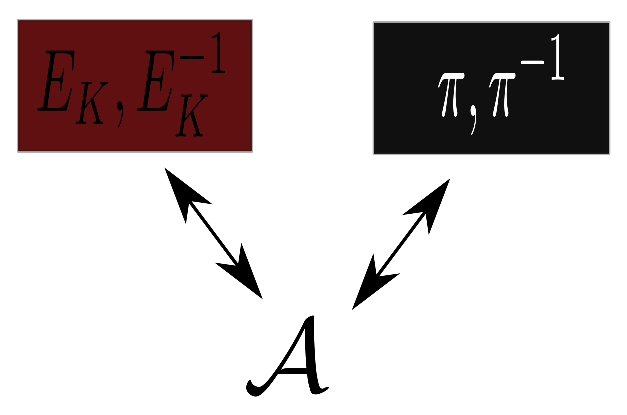
\includegraphics[width=3cm]{images/sprp.eps}

	\end{center}
	\end{column}
	\begin{column}{6cm}
	{\color{red}  $Perm(n)$ es el conjunto de todas las permutaciones $n$ a $n$ bits}.
	\end{column}
	\end{columns}
}

\frame
{
	\frametitle{Funciones \textit{hash} polinomiales}

Informalmente una función \textit{hash} es una función que proyecta una cadena muy grande en un mucho más pequeña. 

En este trabajo utilizamos funciones \textit{hash} polinomiales:

$$ H:\{0,1\}^n \times \{0,1\}^{nm} \rightarrow \{0,1\}^n $$

Definidas como:

$$H_h(P_1||...||P_m) = P_1h^m \oplus P_2h^{m-1} \oplus ... \oplus P_mh$$

Todas las operaciones son en el campo $GF(2^n)$ y $h$, $P_i \in \{0,1\}^n$.
}

\frame
{
	\frametitle{Cajas de Substitución}

\begin{block}{Definición}
Son funciones del tipo $S:\{0,1\}^n\rightarrow \{0,1\}^n$, deben cumplir las siguientes propiedades:

\begin{itemize}
\item No linealidad.
\item Criterio de independencia de bits.
\item Criterio de avalancha.
\item Criterio estricto de avalancha.
\item Criterio de completitud.
\item  lineal y diferencial.
\end{itemize}

\end{block}	
}

\frame
{
	\frametitle{Cajas de Substitución}

\begin{center}
	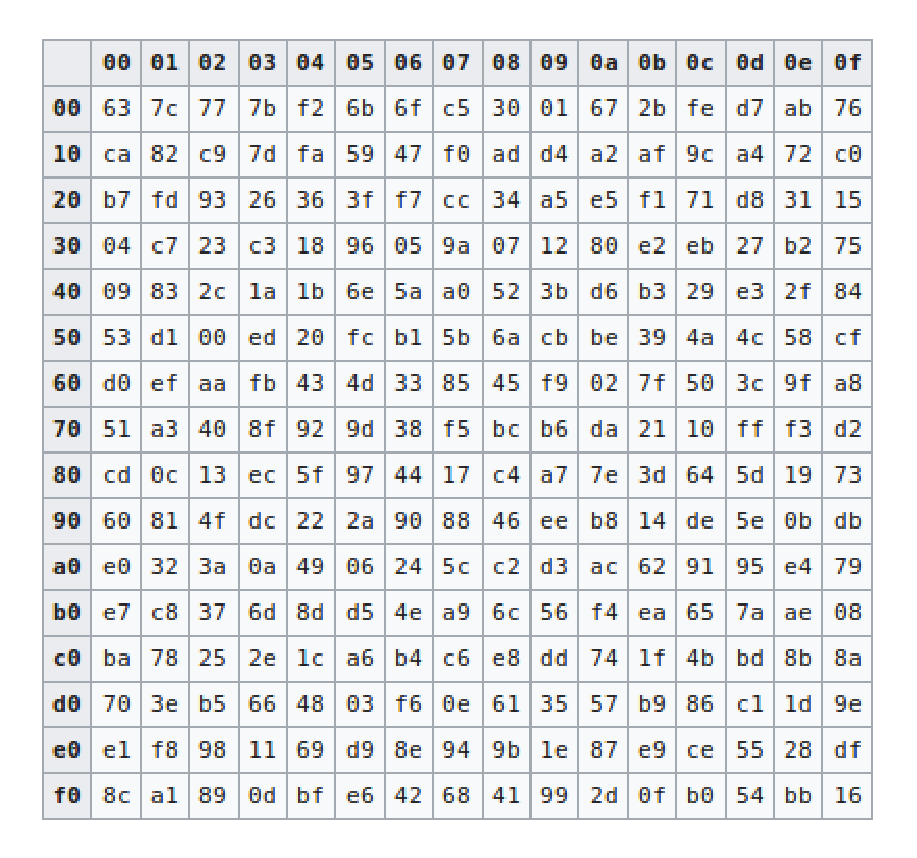
\includegraphics[width=7cm]{images/sbox.eps}

\end{center}

}


\frame
{
	\frametitle{Red de Feistel}
	
	\begin{block}{Definición}
		Es una función iterativa $FN:\{0,1\}^{2t}\times \{0,1\}^k \rightarrow \{0,1\}^{2t}$, definida como:\\
		\vspace{0.5cm}
		$(L_{i-1},R_{i-1})\stackrel{K_i}\rightarrow (L_i,R_i)$,\\
		\vspace{0.5cm}
		$ L_i\leftarrow R_{i-1},R_i \leftarrow L_{i-1} \oplus f(K,R_{i-1})$\\
		\vspace{0.5cm}
		donde:\\
		\vspace{0.5cm}
		$f:\{0,1\}^t \times \{0,1\}^k \rightarrow \{0,1\}^t$		
		
	\end{block}

}

\frame
{
	\frametitle{Red de Feistel}
	
		\begin{center}
	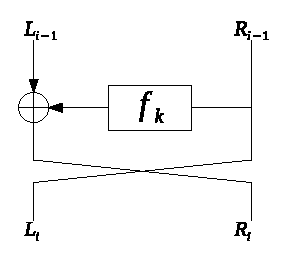
\includegraphics[width=6cm]{images/FN.eps}

	\end{center}
}

\frame
{
	\frametitle{Cifrador basado en redes de Feistel}
	
		\begin{center}
	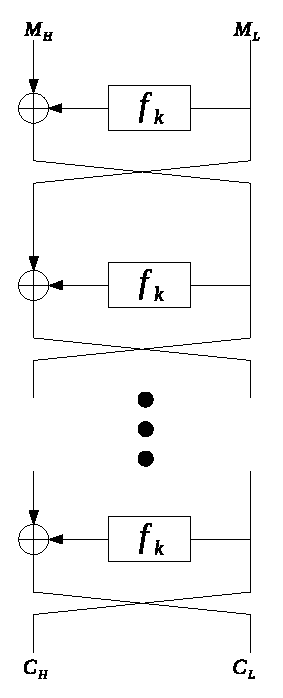
\includegraphics[width=3cm]{images/cipherFN.eps}

	\end{center}
}

\frame
{
	\frametitle{Red de substituciones y permutaciones}

Este tipo de cifradores los podemos considerar como una composición de funciones:

\begin{itemize}
\item Suma de la llave $ADDRK:\{0,1\}^n \times \{0,1\}^n \rightarrow \{0,1\}^n$.
\item $SB:\{0,1\}^n \rightarrow \{0,1\}^n$.
\item $P:\{0,1\}^n \rightarrow \{0,1\}^n$.
\item El cifrador se forma como: $ADDRK \circ SB \circ P$.
\end{itemize}

}

\frame
{
	\frametitle{Red de substituciones y permutaciones}
	
		\begin{center}
	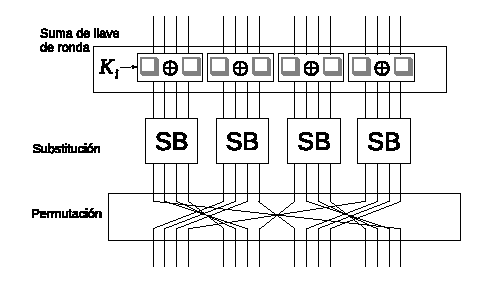
\includegraphics[width=10cm]{images/SPN.eps}

	\end{center}
}

\frame
{
	\frametitle{AES}
	
	$$\{0,1\}^{128} \times \{0,1\}^{128} \rightarrow \{0,1\}^{128}$$
	$$\{0,1\}^{128} \times \{0,1\}^{192} \rightarrow \{0,1\}^{128}$$
	$$\{0,1\}^{128} \times \{0,1\}^{256} \rightarrow \{0,1\}^{128}$$
		
	
	\begin{itemize}
	\item Tamaño de bloque $n=128$, $k=128,192,256$.
	\item Instancía la familia de permutaciones $perm(128)$.\pause
	\item {\color{red} ¿Cuántas instancias?}\pause $2^n!$.
	\item {\color{red} ¿Cuántas se pueden instanciar con $k=128$?}\pause $2^{128}$.
	\item {\color{red} ¿Cuántas se pueden instanciar con $k=192$?}\pause $2^{192}$.
	\item {\color{red} ¿Cuántas se pueden instanciar con $k=256$?}\pause $2^{256}$.
	\item {\color{red} Se pueden instanciar todas?}\pause $2^{256}<2^{128}$.

	\end{itemize}

}


\frame
{
	\frametitle{Cálculo de la caja S de AES}

Se utiliza el campo $GF(2^8)$ definido por $q(x)=x^8+x^4+x^3+x+1$, primero se calcula el inverso multiplicativo.

$$b=a^{-1}$$

{\color{red} Para el cero se proyecta en el mismo.}


\begin{equation*} 
\begin{bmatrix} 
c_7 \\
c_6 \\
c_5 \\
c_4 \\
c_3 \\
c_2 \\
c_1 \\
c_0
\end{bmatrix}
=
\begin{bmatrix} 
1 & 1 & 1 & 1 & 1 & 0 & 0 & 0 \\
0 & 1 & 1 & 1 & 1 & 1 & 0 & 0 \\
0 & 0 & 1 & 1 & 1 & 1 & 1 & 0 \\
0 & 0 & 0 & 1 & 1 & 1 & 1 & 1 \\
1 & 0 & 0 & 0 & 1 & 1 & 1 & 1 \\
1 & 1 & 0 & 0 & 0 & 1 & 1 & 1 \\
1 & 1 & 1 & 0 & 0 & 0 & 1 & 1 \\ 
1 & 1 & 1 & 1 & 0 & 0 & 0 & 1
\end{bmatrix}
\times
\begin{bmatrix}
b_7 \\
b_6 \\
b_5 \\
b_4 \\
b_3 \\
b_2 \\
b_1 \\
b_0 
\end{bmatrix}
\oplus
\begin{bmatrix}
0 \\
1 \\
1 \\
0 \\
0 \\
0 \\
1 \\
1 
\end{bmatrix}
\end{equation*}

}

\frame
{
	\frametitle{Caja S inversa}

Se utiliza el campo $GF(2^8)$ definido por $q(x)=x^8+x^4+x^3+x+1$, primero se calcula el inverso multiplicativo.

\begin{equation*} 
\begin{bmatrix} 
b_7 \\
b_6 \\
b_5 \\
b_4 \\
b_3 \\
b_2 \\
b_1 \\
b_0
\end{bmatrix}
=
\begin{bmatrix} 
0 & 1 & 0 & 1 & 0 & 0 & 1 & 0 \\
0 & 0 & 1 & 0 & 1 & 0 & 0 & 1\\ 
1 & 0 & 0 & 1 & 0 & 1 & 0 & 0 \\ 
0 & 1 & 0 & 0 & 1 & 0 & 1 & 0 \\ 
0 & 0 & 1 & 0 & 0 & 1 & 0 & 1 \\ 
1 & 0 & 0 & 1 & 0 & 0 & 1 & 0 \\ 
0 & 1 & 0 & 0 & 1 & 0 & 0 & 1 \\ 
1 & 0 & 1 & 0 & 0 & 1 & 0 & 0 
\end{bmatrix}
\times
\begin{bmatrix}
c_7 \\
c_6 \\
c_5 \\
c_4 \\
c_3 \\
c_2 \\
c_1 \\
c_0 
\end{bmatrix}
\oplus
\begin{bmatrix}
0 \\
0 \\
0 \\
0 \\
0 \\
1 \\
0 \\
1 
\end{bmatrix}
\end{equation*}

$$a=b^{-1}$$

}

\frame
{
	\frametitle{Reducción en $GF(2^8)$ generado con  $q(x)=x^8+x^4+x^3+x+1$}

	
	\begin{center}
		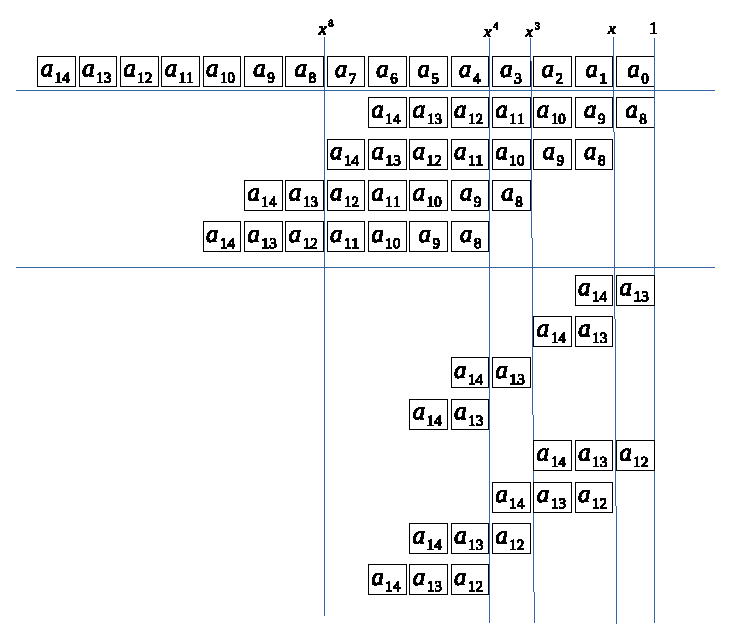
\includegraphics[width=8cm]{images/mulgf8_1.eps}
	\end{center}

}

\frame
{
	\frametitle{Reducción en $GF(2^8)$ generado con  $q(x)=x^8+x^4+x^3+x+1$}

	
	\begin{center}
		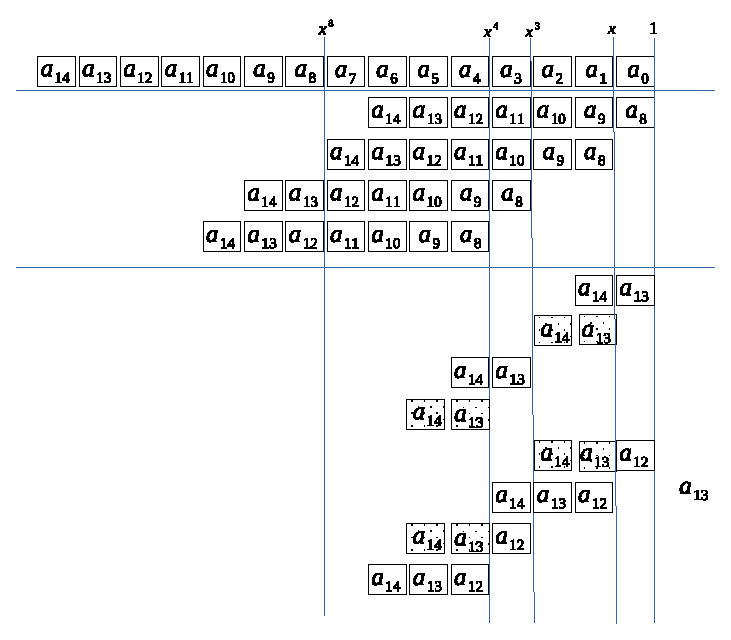
\includegraphics[width=8cm]{images/mulgf8_2.eps}
	\end{center}

}

\frame
{
	\frametitle{Reducción en $GF(2^8)$ generado con  $q(x)=x^8+x^4+x^3+x+1$}

	
	\begin{center}
		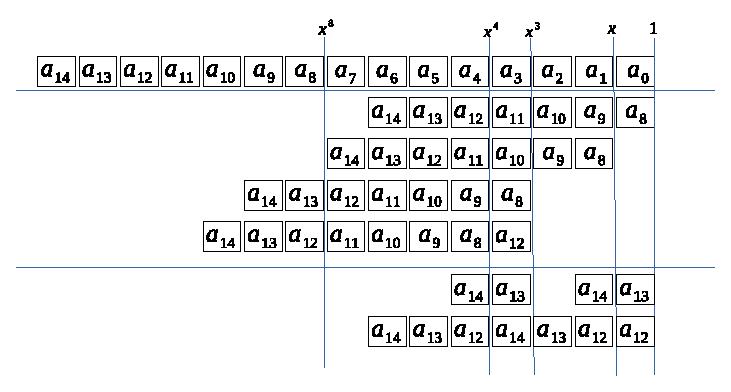
\includegraphics[width=8cm]{images/mulgf8_3.eps}
	\end{center}

}


\frame
{
	\frametitle{Optimización para 32 bits T-Boxes}

Aplicando la sustitución de bytes al estado (previamente ya se aplicó el corrimiento de filas){\color{red} recordar que cambiar el orden de BS y SR no altera el resultado}

\begin{equation*}
\begin{bmatrix} 
A_{11} & A_{12} & A_{13} & A_{14} \\
A_{21} & A_{22} & A_{23} & A_{24} \\
A_{31} & A_{32} & A_{33} & A_{34} \\
A_{41} & A_{42} & A_{43} & A_{44}
\end{bmatrix}
{\stackrel{SB}\rightarrow}
\begin{bmatrix} 
SB(A_{11}) & SB(A_{12}) & SB(A_{13}) & SB(A_{14}) \\
SB(A_{21}) & SB(A_{22}) & SB(A_{23}) & SB(A_{24}) \\
SB(A_{31}) & SB(A_{32}) & SB(A_{33}) & SB(A_{34}) \\
SB(A_{41}) & SB(A_{42}) & SB(A_{43}) & SB(A_{44})  
\end{bmatrix}
\end{equation*}
}

\frame
{
	\frametitle{Optimización para 32 bits T-Boxes}

\begin{equation*}
\begin{bmatrix} 
2 & 3 & 1 & 1 \\
1 & 2 & 3 & 1 \\
1 & 1 & 2 & 3 \\
3 & 1 & 1 & 2 
\end{bmatrix}
\begin{bmatrix} 
SB(A_{11}) & SB(A_{12}) & SB(A_{13}) & SB(A_{14}) \\
SB(A_{21}) & SB(A_{22}) & SB(A_{23}) & SB(A_{24}) \\
SB(A_{31}) & SB(A_{32}) & SB(A_{33}) & SB(A_{34}) \\
SB(A_{41}) & SB(A_{42}) & SB(A_{43}) & SB(A_{44})  
\end{bmatrix}
\end{equation*}
}


\frame
{
	\frametitle{T-Boxes}

\begin{columns}
\begin{column}{4cm}
\begin{equation*}
\begin{bmatrix} 
2 & 3 & 1 & 1 \\
1 & 2 & 3 & 1 \\
1 & 1 & 2 & 3 \\
3 & 1 & 1 & 2 
\end{bmatrix}\times
\begin{bmatrix} 
SB(A_{11}) \\
SB(A_{21}) \\
SB(A_{31}) \\
SB(A_{41})  
\end{bmatrix}
\end{equation*}\\

\begin{equation*}
\begin{bmatrix} 
2 & 3 & 1 & 1 \\
1 & 2 & 3 & 1 \\
1 & 1 & 2 & 3 \\
3 & 1 & 1 & 2 
\end{bmatrix}\times
\begin{bmatrix} 
SB(A_{12}) \\
SB(A_{22}) \\
SB(A_{32}) \\
SB(A_{42})   
\end{bmatrix}
\end{equation*}



\end{column}
\begin{column}{4cm}	
\begin{equation*}
\begin{bmatrix} 
2 & 3 & 1 & 1 \\
1 & 2 & 3 & 1 \\
1 & 1 & 2 & 3 \\
3 & 1 & 1 & 2 
\end{bmatrix}\times
\begin{bmatrix} 
SB(A_{13})\\
SB(A_{23})\\
SB(A_{33})\\
SB(A_{43})  
\end{bmatrix}
\end{equation*}\\

\begin{equation*}	
\begin{bmatrix} 
2 & 3 & 1 & 1 \\
1 & 2 & 3 & 1 \\
1 & 1 & 2 & 3 \\
3 & 1 & 1 & 2 
\end{bmatrix}\times
\begin{bmatrix} 
SB(A_{14}) \\
SB(A_{24}) \\
SB(A_{34}) \\
SB(A_{44})  
\end{bmatrix}
\end{equation*}
\end{column}
\end{columns}
	
}

\frame
{
	\frametitle{T-Boxes}
\tiny

\begin{tabular}{|ccccccc|}
$2SB(A_{11})$ & $\oplus$ & $3SB(A_{21})$ & $\oplus$ & $ SB(A_{31})$ & $\oplus$ & $ SB(A_{41})$\\
$ SB(A_{11})$ & $\oplus$ & $2SB(A_{21})$ & $\oplus$ & $3SB(A_{31})$ & $\oplus$ & $ SB(A_{41})$ \\
$ SB(A_{11})$ & $\oplus$ & $ SB(A_{21})$ & $\oplus$ & $2SB(A_{31})$ & $\oplus$ & $3SB(A_{41})$ \\
$3SB(A_{11})$ & $\oplus$ & $ SB(A_{21})$ & $\oplus$ & $ SB(A_{31})$ & $\oplus$ & $2SB(A_{41})$ 
\end{tabular}1 000 1 1 1 1
\vspace{0.5cm}

\begin{tabular}{|ccccccc|}
$2SB(A_{12})$ & $\oplus$ & $3SB(A_{22})$ & $\oplus$ & $ SB(A_{32})$ & $\oplus$ & $ SB(A_{42})$\\
$ SB(A_{12})$ & $\oplus$ & $2SB(A_{22})$ & $\oplus$ & $3SB(A_{32})$ & $\oplus$ & $ SB(A_{42})$ \\
$ SB(A_{12})$ & $\oplus$ & $ SB(A_{22})$ & $\oplus$ & $2SB(A_{32})$ & $\oplus$ & $3SB(A_{42})$ \\
$3SB(A_{12})$ & $\oplus$ & $ SB(A_{22})$ & $\oplus$ & $ SB(A_{32})$ & $\oplus$ & $2SB(A_{42})$ 
\end{tabular}
\vspace{0.5cm}

\begin{tabular}{|ccccccc|}
$2SB(A_{13})$ & $\oplus$ & $3SB(A_{23})$ & $\oplus$ & $ SB(A_{33})$ & $\oplus$ & $ SB(A_{43})$\\
$ SB(A_{13})$ & $\oplus$ & $2SB(A_{23})$ & $\oplus$ & $3SB(A_{33})$ & $\oplus$ & $ SB(A_{43})$ \\
$ SB(A_{13})$ & $\oplus$ & $ SB(A_{23})$ & $\oplus$ & $2SB(A_{33})$ & $\oplus$ & $3SB(A_{43})$ \\
$3SB(A_{13})$ & $\oplus$ & $ SB(A_{23})$ & $\oplus$ & $ SB(A_{33})$ & $\oplus$ & $2SB(A_{43})$ 
\end{tabular}
\vspace{0.5cm}

\begin{tabular}{|ccccccc|}
$2SB(A_{14})$ & $\oplus$ & $3SB(A_{24})$ & $\oplus$ & $ SB(A_{34})$ & $\oplus$ & $ SB(A_{44})$\\
$ SB(A_{14})$ & $\oplus$ & $2SB(A_{24})$ & $\oplus$ & $3SB(A_{34})$ & $\oplus$ & $ SB(A_{44})$ \\
$ SB(A_{14})$ & $\oplus$ & $ SB(A_{24})$ & $\oplus$ & $2SB(A_{34})$ & $\oplus$ & $3SB(A_{44})$ \\
$3SB(A_{14})$ & $\oplus$ & $ SB(A_{24})$ & $\oplus$ & $ SB(A_{34})$ & $\oplus$ & $2SB(A_{44})$ 
\end{tabular}


}


\frame
{
	\frametitle{T-Boxes}

\begin{columns}
\begin{column}{4cm}
\begin{equation*}
T_1=\begin{bmatrix} 
2SB(x)\\
SB(x)\\
SB(x)\\
3SB(x)
\end{bmatrix}
\end{equation*}
\vspace{0.5cm}
\begin{equation*}
T_2=\begin{bmatrix} 
3SB(x)\\
2SB(x)\\
SB(x)\\
SB(x)
\end{bmatrix}
\end{equation*}
\end{column}
\begin{column}{4cm}	
\begin{equation*}
T_3=\begin{bmatrix} 
SB(x)\\
3SB(x)\\
2SB(x)\\
SB(x)
\end{bmatrix}
\end{equation*}
\vspace{0.5cm}
\begin{equation*}
T_4=\begin{bmatrix} 
SB(x)\\
SB(x)\\
3SB(x)\\
2SB(x)
\end{bmatrix}
\end{equation*}
\end{column}
\end{columns}
	
\vspace{0.5cm}
	{\color{red}Para calcular el MC para una columna:
	
	$$ MC_i = T_1 \oplus T_2 \oplus T_3 \oplus T_4$$
	
	
	}	
	
	
	
}

\frame
{
	\frametitle{Modos de operación de cifradores por bloques}

Los cifradores por bloques sólo pueden cifrar $n$ bits, en la realidad los mensajes tendrían las siguientes características:


\begin{itemize}
\item En general mucho más grandes que $n$.
\item $\{0,1\}^*$ el espacio de mensajes deben ser todas las cadenas binarias.
\item Pueden ser incluso un sólo bit. \pause
\item {\color{red}Para extender el dominio de un cifrador por bloques se utiliza un modo de operación}.
\end{itemize}

}

\frame
{
	\frametitle{Tipos de modos de operación}

\begin{itemize}
\item Sólo cifrado: \pause {\color{blue} Ofrecen privacidad de la información, es decir sólo los poseedores de la llave secreta pueden tener acceso a ella.}\pause
\item Códigos de autenticación de mensajes: \pause {\color{blue} Ofrecen autenticación de la fuente que envía el mensaje, ya que solamente los poseedores de la llave secreta podrán obtener la misma etiqueta de autenticación, adicionalmente proporcionan integridad de datos ya que pueden detectar cambios hechos al mensaje durante la transmisión.}

\item Cifrado autenticado: \pause {\color{blue}Ofrecen los dos servicios anteriormente mencionados, es decir privacidad y autenticación.}

\item Cifrado que preserva la longitud: \pause {\color{blue}En ocasiones no es posible guardar información extra, es decir, el mensaje cifrado debe ser exactamente de la longitud del mensaje original.} 
\end{itemize}
}

\frame
{
	\frametitle{Modos de operación de sólo cifrado}

	Formalmente son funciones del tipo:\\
	
	$\textbf{E}:\{0,1\}^*\times \{0,1\}^k \rightarrow \{0,1\}^*$
	
	\begin{itemize}
	\item $\{0,1\}^*$ es el espacio de mensajes.
	\item $\{0,1\}^k$.
	\item Se construyen cifradores por bloques que procesan $n$ bits y algunas operaciones en $GF(2^n)$. 
	\end{itemize}
	
}



\frame
{
	\frametitle{Modos de operación tradicionales}

\begin{columns}[c]

\column{2in}
{
\center
\framebox{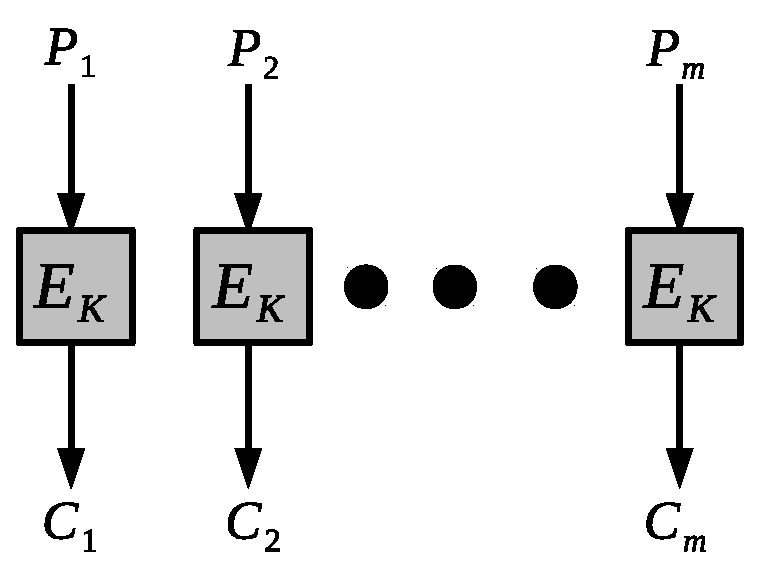
\includegraphics[width=3cm]{images/ecb.eps}}\\
Electronic Code Book (ECB)\\
\vspace{1cm}
\framebox{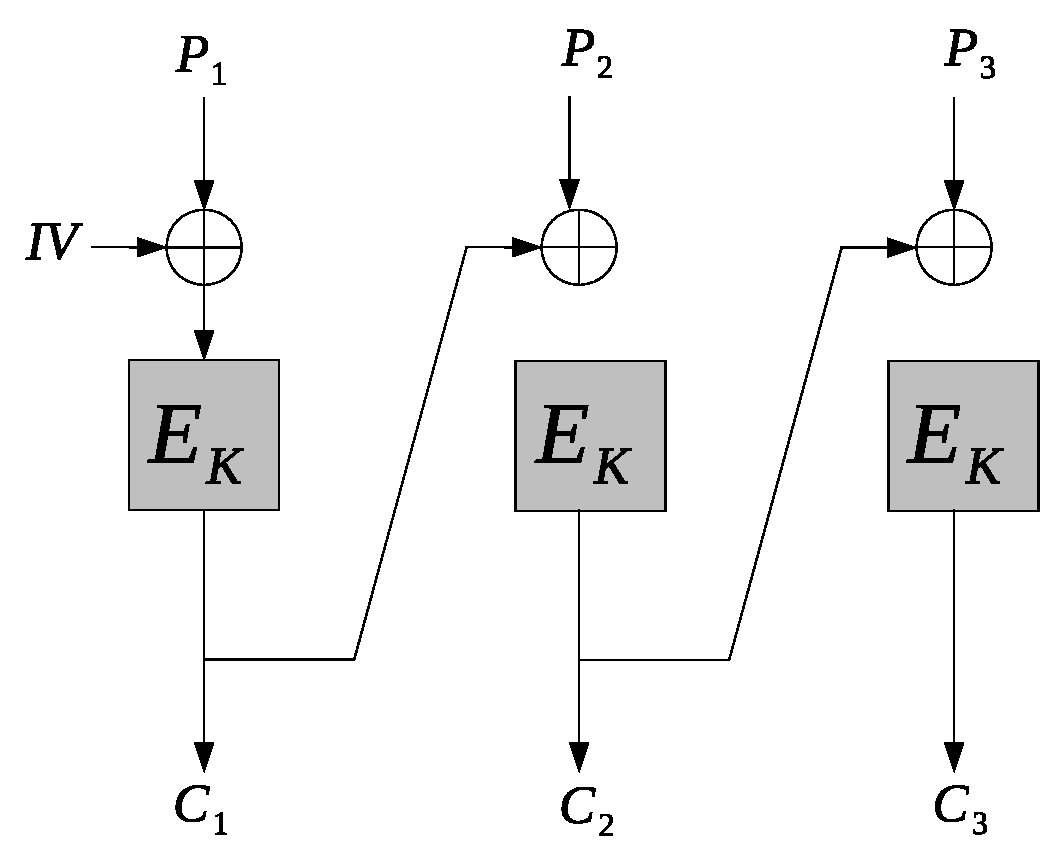
\includegraphics[width=3cm]{images/CBC.eps}}\\
Cipher Block Chaining (CBC)\\
}
\column{2in}
{
\center
\framebox{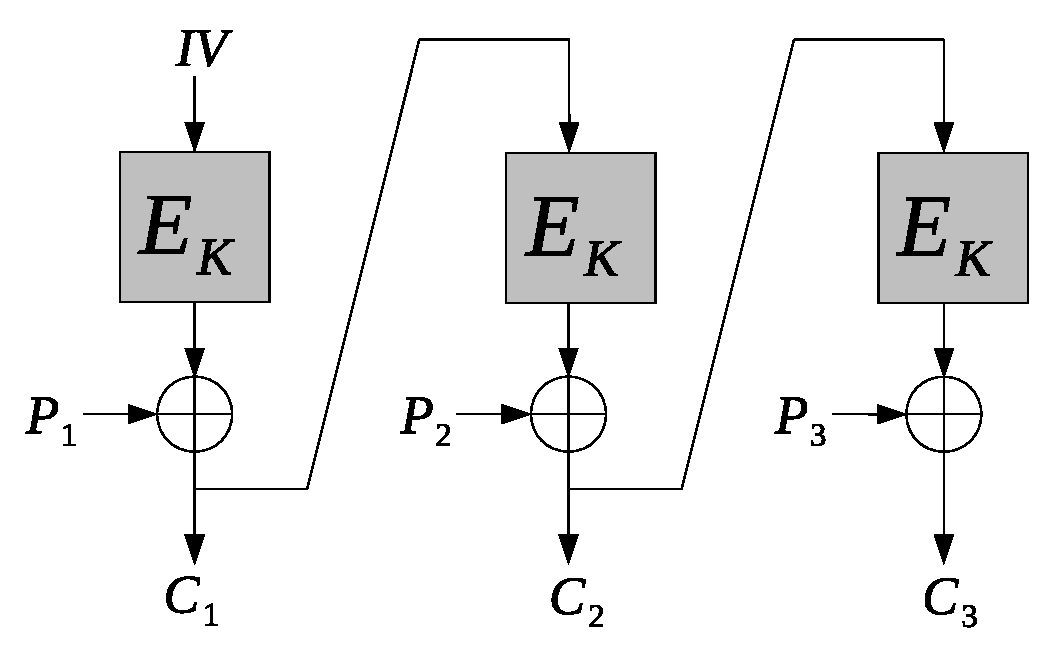
\includegraphics[width=4cm]{images/CFB.eps}}\\
Cipher Feedback (CFB)\\
\vspace{1cm}

\framebox{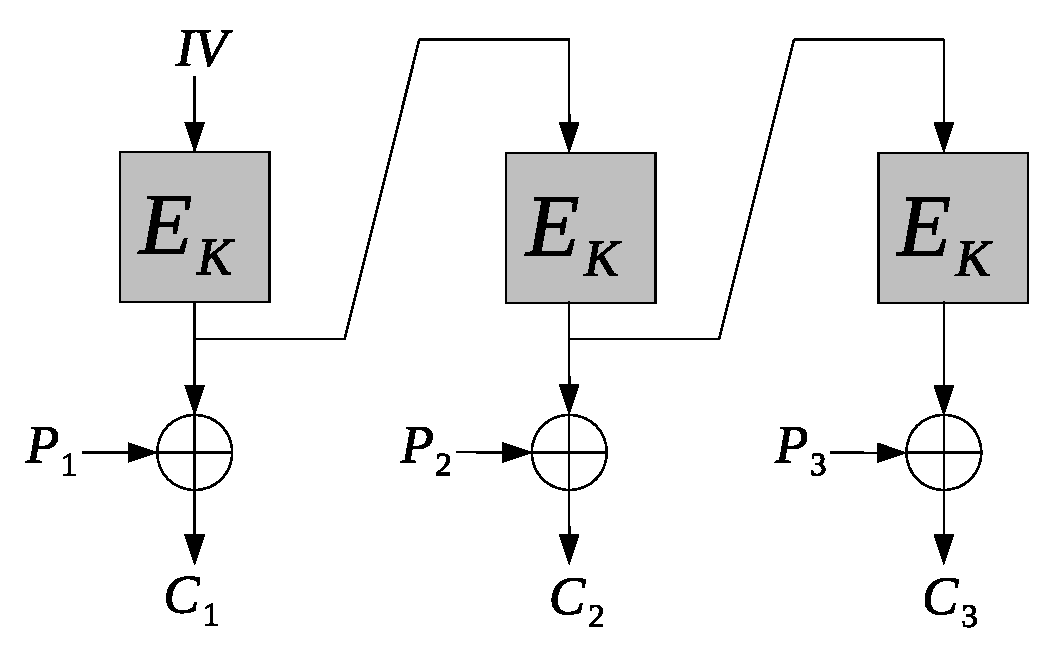
\includegraphics[width=4cm]{images/OFB.eps}}\\
Output Feedback (OFB)\\
}

\end{columns}

}

\frame
{
	\frametitle{Modo contador}

\begin{columns}[c]

\column{2in}
{

\center
\framebox{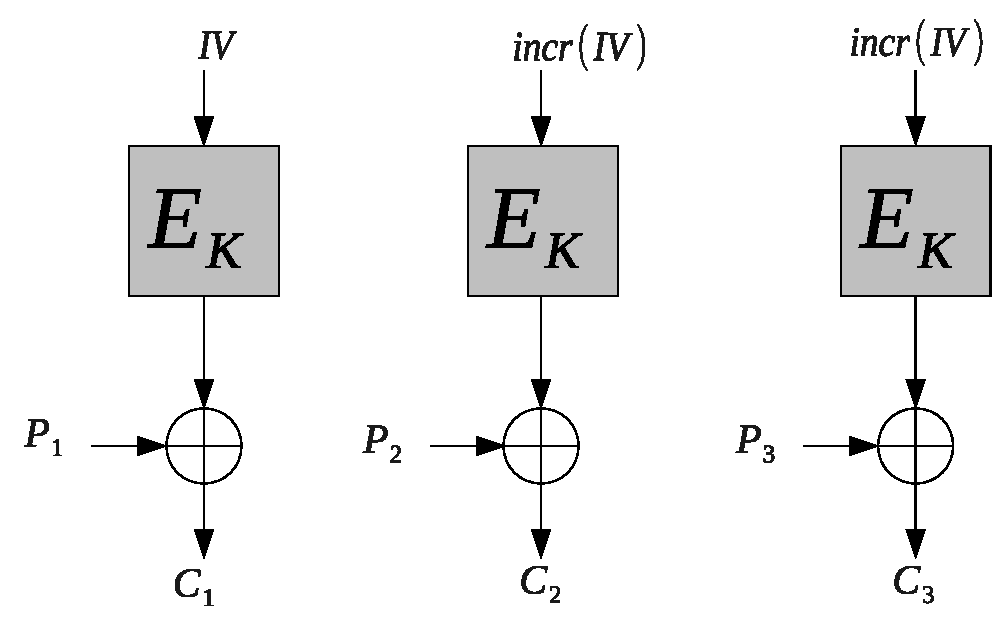
\includegraphics[width=5cm]{images/ctr.eps}}\\
Counter mode incremental (Ctr)\\

}
\column{2in}
{
\center
\framebox{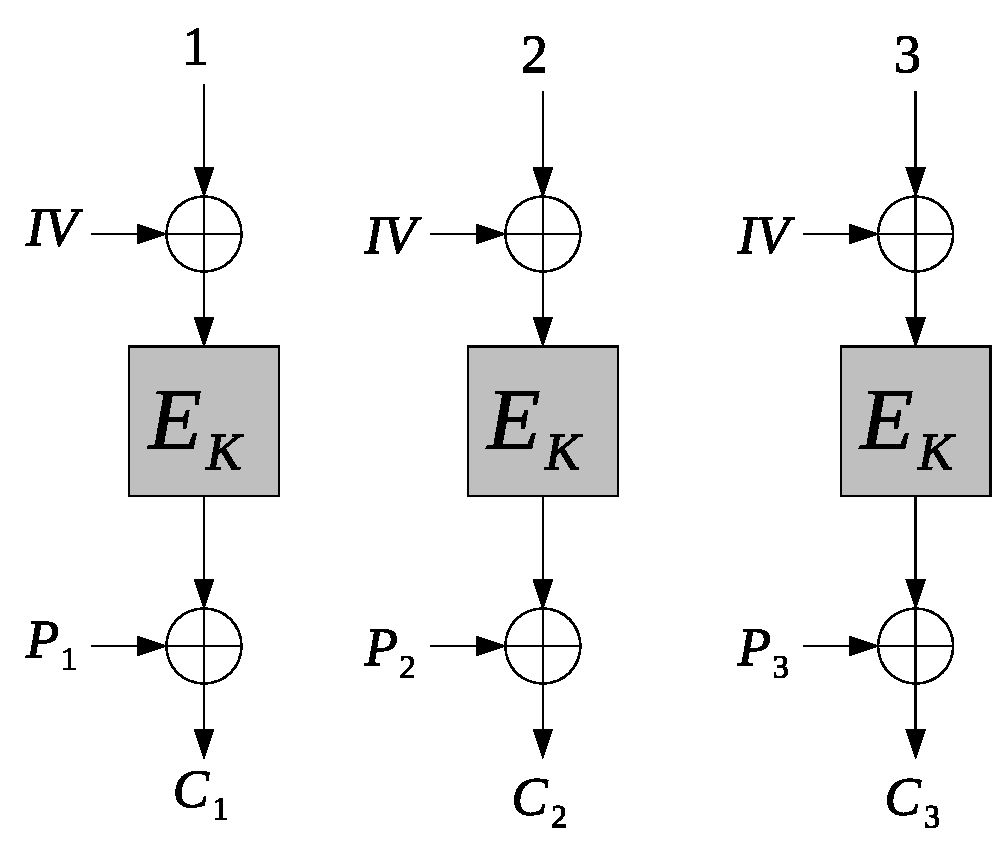
\includegraphics[width=4cm]{images/ctr_xor.eps}}\\
Counter Mode Xor (Ctr\_$\oplus$)\\

}

\end{columns}

}


\frame
{
	\frametitle{Cipher Block Chaining (CBC)}

\begin{columns}
\begin{column}{4cm}
\framebox{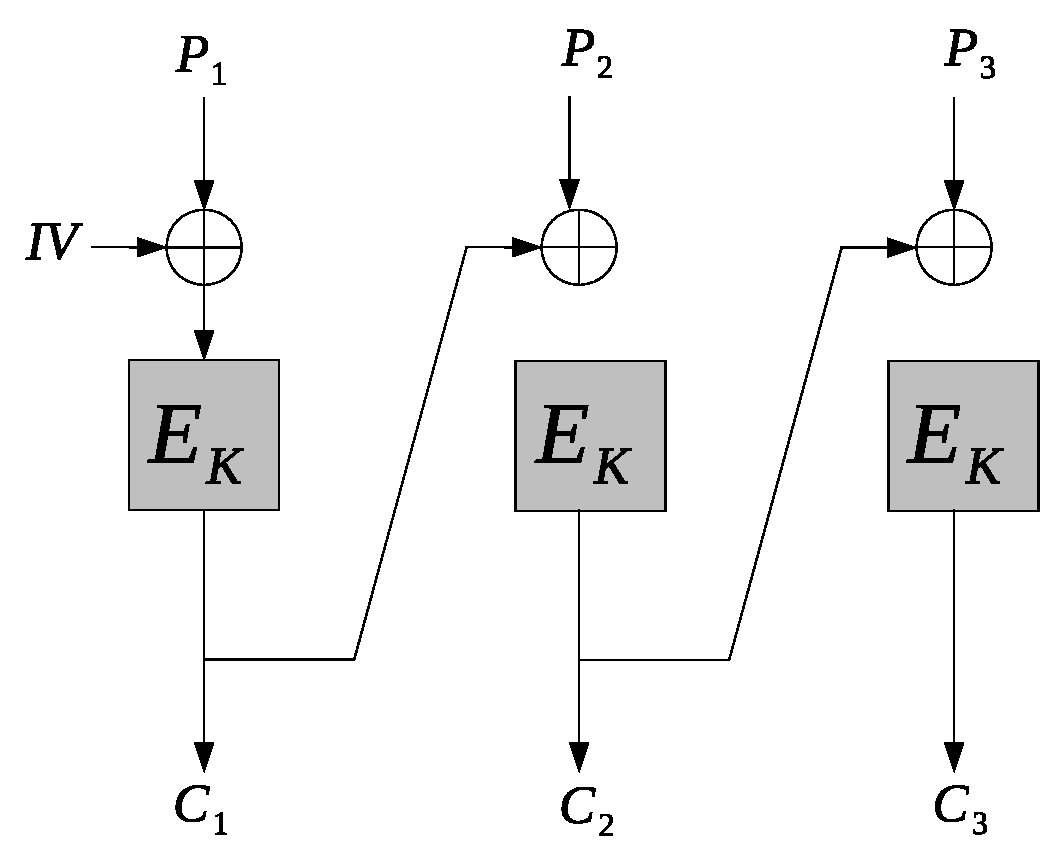
\includegraphics[width=4cm]{images/CBC.eps}}\\

\end{column}
\begin{column}{4cm}	
$C_1\leftarrow E_K(IV\oplus P_1)$\\
$C_2\leftarrow E_K(C_1\oplus P_2)$\\
$C_3\leftarrow E_K(C_2\oplus P_3)$\\
\vspace{2cm}
$P_1\leftarrow E^{-1}_K(C_1)\oplus IV$\\
$P_2\leftarrow E^{-1}_K(C_2)\oplus C_1$\\
$P_3\leftarrow E^{-1}_K(C_3)\oplus C_2$\\

\end{column}
\end{columns}
	
	
}


\frame
{
	\frametitle{Cipher Feedback (CFB)}

\begin{columns}
\begin{column}{4cm}
\framebox{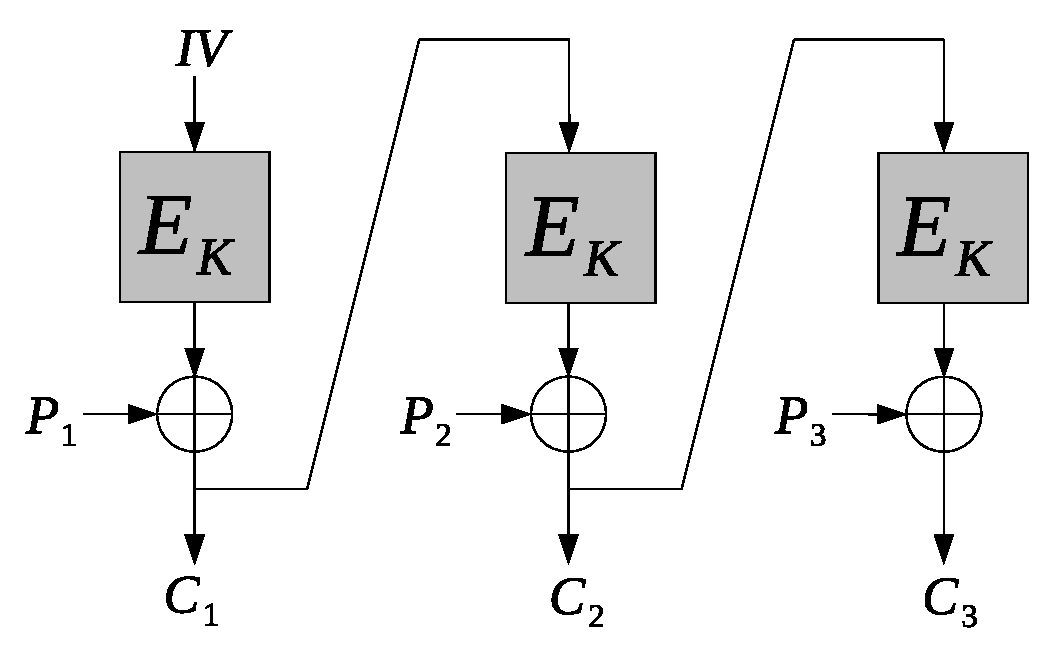
\includegraphics[width=4cm]{images/CFB.eps}}\\
\end{column}
\begin{column}{4cm}	
$C_1\leftarrow E_K(IV)\oplus P_1$\\
$C_2\leftarrow E_K(C_1)\oplus P_2$\\
$C_3\leftarrow E_K(C_2)\oplus P_3$\\
\vspace{2cm}
$P_1\leftarrow E_K(IV)\oplus C_1$\\
$P_2\leftarrow E_K(C_1)\oplus C_2$\\
$P_3\leftarrow E_K(C_2)\oplus C_3$\\

\end{column}
\end{columns}

}

\frame
{
	\frametitle{Output Feedback (OFB)}

\begin{columns}
\begin{column}{4cm}
\framebox{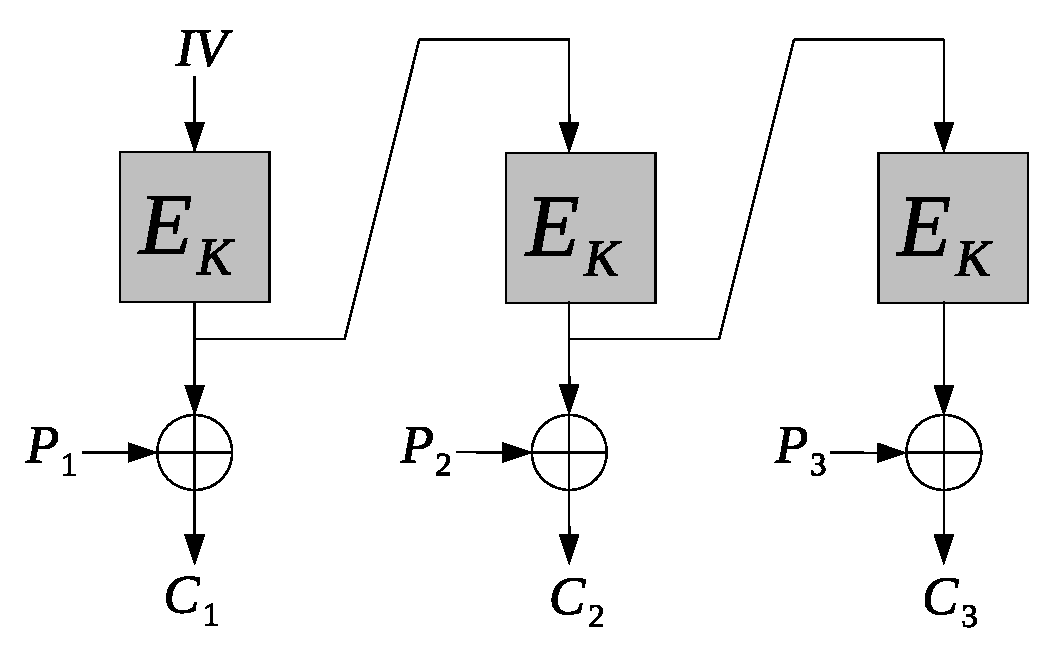
\includegraphics[width=4cm]{images/OFB.eps}}\\
\end{column}
\begin{column}{4cm}	
{\footnotesize
$R_1\leftarrow E_K(IV);  C_1\leftarrow R_1 \oplus P_1$\\
$R_2\leftarrow E_K(R_1); C_2\leftarrow R_2 \oplus P_2$\\
$R_3\leftarrow E_K(R_2); C_3\leftarrow R_3 \oplus P_3$\\
\vspace{2cm}
$R_1\leftarrow E_K(IV);  P_1\leftarrow R_1 \oplus C_1$\\
$R_2\leftarrow E_K(R_1); P_2\leftarrow R_2 \oplus C_2$\\
$R_3\leftarrow E_K(R_2); P_3\leftarrow R_3 \oplus C_3$\\

}
\end{column}
\end{columns}

}

\frame
{
	\frametitle{Counter mode incremental (Ctr)}

\begin{columns}
\begin{column}{4cm}
\framebox{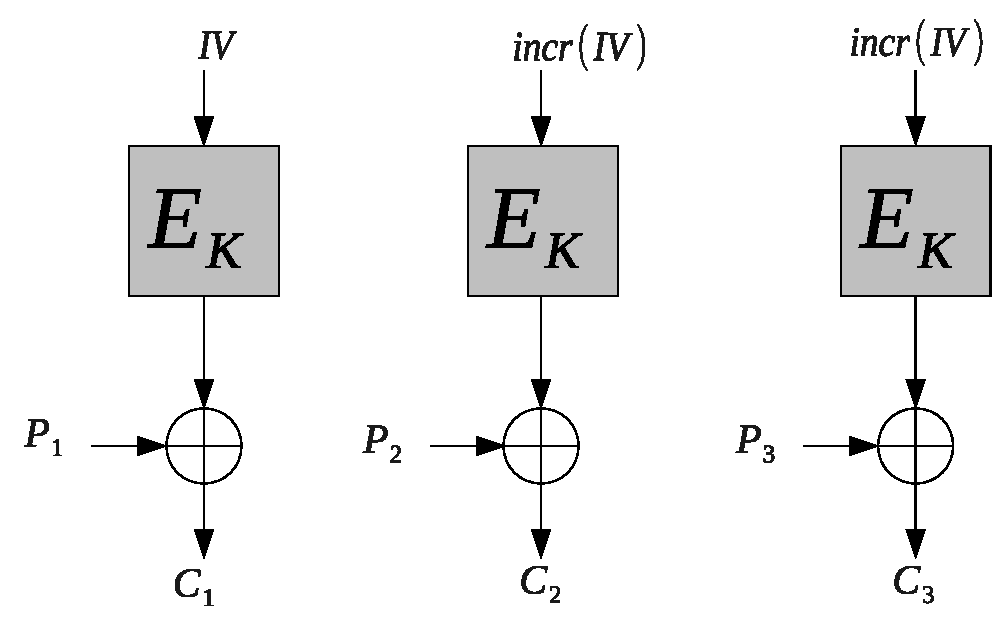
\includegraphics[width=5cm]{images/ctr.eps}}\\

$$inc(IV) \leftarrow IV++$$

\end{column}
\begin{column}{4cm}	
{\footnotesize
$R_1\leftarrow E_K(IV)$; \\ $C_1\leftarrow R_1 \oplus P_1$\\
\vspace{0.2cm}
$R_2\leftarrow E_K(icr(IV))$;\\ $C_2\leftarrow R_2 \oplus P_2$\\
\vspace{0.2cm}
$R_3\leftarrow E_K(icr(IV))$;\\ $C_3\leftarrow R_3 \oplus P_3$\\
\vspace{1cm}
$R_1\leftarrow E_K(IV)$;\\  $P_1\leftarrow R_1 \oplus C_1$\\
\vspace{0.2cm}
$R_2\leftarrow E_K(icr(IV))$;\\ $P_2\leftarrow R_2 \oplus C_2$\\
\vspace{0.2cm}
$R_3\leftarrow E_K(icr(IV))$;\\ $P_3\leftarrow R_3 \oplus C_3$\\
}
\end{column}
\end{columns}

}

\frame
{
	\frametitle{Ataques de recuperación de la llave contra cifradores por bloque}
	\begin{block}{Fijando un cifrador por bloques }
	\begin{center}
	\bc
	\end{center}
	\begin{itemize}
	\item tamaño de llave $k$.
	\item tamaño de bloque $n$.
	\end{itemize}
	\end{block}
	\vspace{0.5cm}
	{\color{red}
	Históricamente el criptanálisis de cifradores por bloques se ha centrado en recuperar la llave secreta.}
	}

\frame
{
	\frametitle{Ataques de recuperación de la llave contra cifradores por bloque}
	
	 Dicho ataque puede describirse como sigue:\\
	
	\begin{itemize}
	\item Se elige llave objetivo $T\rand \binStr^k $.
	\item  El adversario posee $q$ pares de entradas/salidas válidas obtenidas de $E_T$:\\         $$(M_1,C_1),(M_2,C_2),...,(M_q,C_q)$$, donde $C_i=E_T(M_i)$ para $i=1,...,q$ y $M_1,...,M_q$ son cadenas binarias de $n$ bits diferentes entre sí. 
	\item El adversario debe encontrar la llave objetivo $T$.
	\end{itemize}		 
}

\frame
{
	Decimos que la lleve $T$ es consistente con los ejemplos de entrada $(M_1,C_1),(M_2,C_2),...,(M_q,C_q)$, si $E_K(M_i)=C_i$ para todo $1\leq i \leq q$.\\
	\vspace{0.5cm}
	Sea $\mathbf{CONS}_E((M_1,C_1),(M_2,C_2),...,(M_q,C_q))$ es conjunto de todas las llaves consistentes con dichas parejas, la llave $T$ está en el conjunto pero dicho conjunto puede ser más grande y contener más llaves.
	
	Para cifradores por bloque reales, se espera que utilizando pocos pares $(M_i,C_i)$ el tamaño del conjunto de posibles llaves sea $1$.

}


\frame
{
	\frametitle{Ataque de mensaje seleccionado}

	$M_1,M_2,...,M_q$ son seleccionados por el adversario, incluso de manera adaptativa. Esto representa que el adversario tiene acceso a $E_K$ en forma de oráculo. 
	
\begin{center}
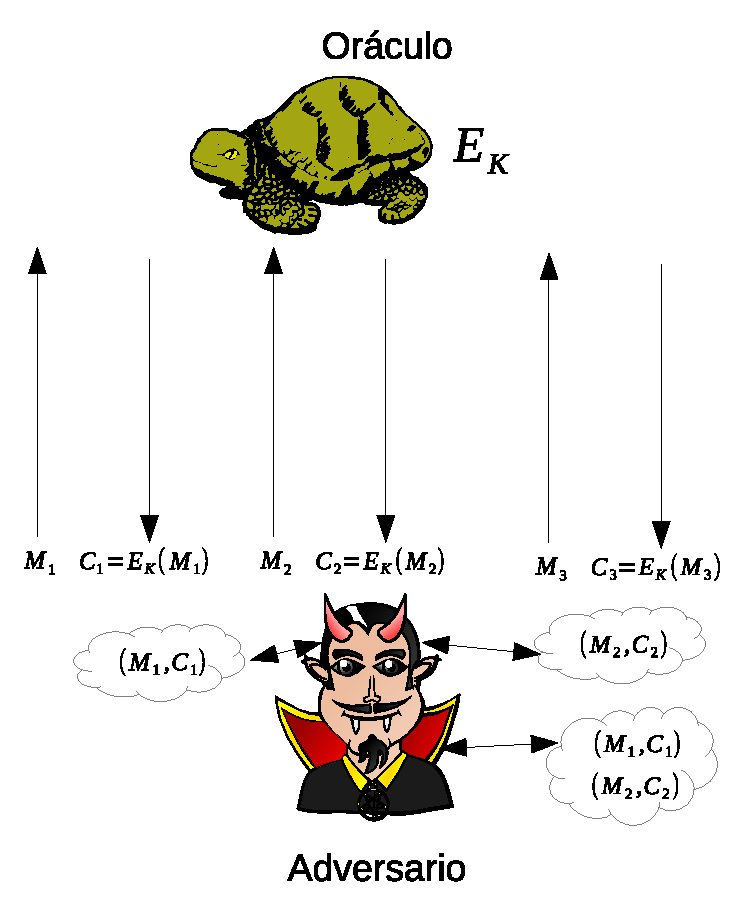
\includegraphics[width=5cm]{images/cma.eps}\\

\end{center}	
}

\frame
{
	\frametitle{Búsqueda exhaustiva de la llave}

	El ataque de mensaje seleccionado es poco realista en la practica por lo que el ataque más obvio es buscar la llave de manera exhaustiva. 
	
	\begin{itemize}
	\item El adversario puede probar todas las posibles llaves en $\binStr^K$ hasta que encuentre la que genere todos los pares $(M_1,C_1),(M_2,C_2),...,(M_q,C_q)$.
	\end{itemize}
\vspace{0.5cm}

	 \begin{tabular}{l}
	 \textbf{Algoritmo} $EKS_E(M_1,C_1)$\\
	 \tab\textbf{for} $i=1,...,2^k$ \textbf{do}\\
	 \tab\tab \textbf{if} $E_{T_i}(M_1)=C_1$ \textbf{then} \textbf{return} $T_i$\\
	 \end{tabular}\\
\vspace{0.5cm}
{\color{red}$T_i$ es la $i-th$ cadena de $k$ bits, en orden lexicográfico.}
}

\frame
{
	\frametitle{Búsqueda exhaustiva de la llave}


	\begin{itemize}
	\item Se puede aumentar la efectividad probando más pares.
	\end{itemize}
\vspace{0.5cm}

	 \begin{tabular}{l}
	 \textbf{Algoritmo} $EKS_E((M_1,C_1),(M_2,C_2),...,(M_q,C_q))$\\
	 \tab\textbf{for} $i=1,...,2^k$ \textbf{do}\\
	 \tab\tab \textbf{if} $E_{T_i}(M_1)=C_1$ \textbf{and} $E_{T_i}(M_2)=C_2$ \\ \tab\tab\textbf{and}...\textbf{and} $E_{T_i}(M_q)=C_q$\textbf{then} \textbf{return} $T_i$\\
	 \end{tabular}\\
\vspace{0.5cm}
{\color{red}Generalmente un valor pequeño de $q$ es suficiente, algo mayor a $k/n$. Para DES, $q=1$ y $q=2$ es suficiente.}
}

\frame
{
	\frametitle{¿Cuánto tiempo lleva la búsqueda exhaustiva de la llave?}

{\color{blue}Un buen cifrador por bloques es diseñado para hacer dicha tarea prohibitiva computacionalmente hablando.}

\begin{itemize}
\item En el peor caso se harían $2^k$ ejecuciones del cifrador por bloques.
\item Si se tiene suerte pueden requerirse mucho menos ejecuciones.
\item Por ejemplo si se encuentra en la primera mitad del espacio de búqueda, sólo se ocuparían $2^{k-1}$ ejecuciones.
\item La medida más adecuada es tomar el promedio.
\end{itemize}

}


\frame
{
	\frametitle{¿Cuánto tiempo lleva la búsqueda exhaustiva de la llave?}

	$$\sum_{i=1}^{2^k} i \cdot Pr\left[ K=T_i \right]= \sum_{i=1}^{2^k} \frac{i}{2^k}$$
	
	$$\frac{1}{2^k} \cdot \sum_{i=1}^{2^k}i=\frac{1}{2^k}\cdot \frac{2^k(2^k+1)}{2}$$	
	
	$$\frac{2^k+1}{2} \approx 2^{k-1} $$
	\pause
	{\color{red}Esto es proque $T_i$ es seleccionada de manera aleatoria con una probabilidad $1/2^k$ de ser $T_i$, y en el caso del ataque se utilizan $i$ ejecuciones de $E$.}
	
}

\frame
{
	\frametitle{Caso práctico DES}

	\begin{itemize}
	\item Utilizando chips que pueden calcular DES con una velocidad de 1.6 Gbps.
	\item Cada bloque de DES es de $64$ bits, el chip puede calcular $(1.6\times 10^9)/64=2.5\times 10^{7}$ ejecuciones de DES por segundo.
	\item Para realizar $2^{55}$ ejecuciones de DES, $|k|=56$. Se requieren $2^{55}/(2.5\times 10^7)\approx 1.44\times 10^9$ segundos.\pause
	\item 45.7 años.
	\end{itemize}
	
	{\color{purple} Para hacer difícil computacionalmente la búsqueda exhaustiva de la llave, hay que tener una longitud de llave adecuada.}

}

\frame
{
	\frametitle{¿Mejores ataques?}
	\pause
	\begin{itemize}
	\item La búsqueda exhaustiva es una ataque genérico y funciona contra cualquier cifrador por bloques, no toma ventaja alguna del funcionamiento interno de los cifradores.
	\item Criptanálisis diferencial puede encontrar una llave de DES usando $2^{47}$ pares $(M_i,C_i)$ ($q=2^{47}$) en un ataque de mensaje seleccionado.
	\item Criptanálisis lineal mejora los resultados del diferencial en dos aspectos. El número de pares $(M_i,C_i)$ se reduce a $2^{44}$, sólo requiere un ataque del tipo de mensaje conocido (no tiene control sobre la selección de ellos).
	\item Criptanálisis algebráico, ataques de boomerang, {\color{red}ataques por canales laterales}. 
	\end{itemize}
}

\frame{
	\frametitle{Esquema de cifrado de llave secreta}

\begin{block}{Definición}
Los denotamos como $\mathcal{SE}(\cal K,E,D)$, consiste de tres algoritmos:


\begin{itemize}
	\item El algoritmo aleatorizado de generación de llaves $\cal K$. $K\rand {\cal K}$, donde ${\cal K}=\binStr^K$ y $K$ es la longitud en bits de la llave.
	\item El algoritmo de cifrado $\cal E$, puede ser alearizado o puede mantener un estado. Toma como entrada una llave de $\cal K$ y un mensaje $M\in\binStr^*$ y regresa el mensaje cifrado $C\in\binStr^*\cup \{\perp\}$. Se denota como $C\rand {\cal E}_K(M)$.
	
	\item Algoritmo determinístico de descifrado $\cal D$, toma la llave $K\in\cal K$ y el mensaje cifrado $C\in \binStr^*$ y entrega $M\in \binStr^*\cup \perp$. Se denota como $M\leftarrow {\cal D}_K(C)$.

\end{itemize}
\end{block}
}

\frame
{
	\frametitle{Indistinguibilidad bajo un ataque de texto en claro seleccionado}

	Se considera que el adversario no conoce la llave secreta.

	\begin{enumerate}
	\item Selecciona dos mensajes de la misma longitud.
	\item Uno de los dos mensajes es cifrado por y el resultado le es entregado.
	\item El adversario tienen que decir que cuál dos los dos mensajes fue el que se cifró. 
	\end{enumerate}
\pause
{\color{red}El esquema es considerado seguro si el adversario toma un tiempo prohibitivo para decir que mensaje fue cifrado.}\\
\vspace{0.5cm}
{\color{red} {¿cuál es la probabilidad mínima de éxito del adversario?}}\\
\pause
\vspace{0.5cm}
{\color{blue}$Pr[adv=>1]=1/2$}
}


\frame
{
	\frametitle{Experimento LR}

	 \begin{tabular}{l}
	 \textbf{Oráculo} ${\cal E}_K(LR(M_0,M_1,b))$ {\color{green}\{$b\in\{0,1\}$, $M_0,M_1\in \binStr^*$\}}  \\
	 \tab\textbf{if} $|M_0|\neq |M_1|$ \textbf{return} $\perp$ \\
	 \tab\tab $C\rand {\cal E}_K(M_b)$\\
	 \tab\tab \textbf{return} C
	 \end{tabular}\\
\vspace{0.5cm}
{\color{red}Experimento \textit{Left or Right}, para un ataque \textit{IND-CPA}.}
}

\frame
{

	\frametitle{Ambos experimentos}

\begin{columns}
\begin{column}{4cm}

	 \begin{tabular}{l}
	 $\mathbf{Exp}_{\cal SE}^{in-cpa-1}$ \\
	 \tab $K\in {\cal K}$\\
	 \tab $d\rand A^{{\cal E}_K(LR(\cdot,\cdot,1))}$\\
	 \tab \textbf{return} d\\
	 \end{tabular}\\

\end{column}
\begin{column}{4cm}	
	 \begin{tabular}{l}
	 $\mathbf{Exp}_{\cal SE}^{in-cpa-0}$ \\
	 \tab $K\in {\cal K}$\\
	 \tab $d\rand A^{{\cal E}_K(LR(\cdot,\cdot,0))}$\\
	 \tab \textbf{return} d\\
	 \end{tabular}\\
\end{column}
\end{columns}

}

\frame
{
	
\frametitle{Seguridad de ECB}
\begin{columns}
\begin{column}{5cm}
	 \begin{tabular}{l}
	 \textbf{Adversario} $A^{{\cal E}_K(LR(\cdot,\cdot,b))}$ \\
	 \tab $M_1\leftarrow 0^{2n}$;$M_0\leftarrow 0^n||1^n$\\
	 \tab $C[1]C[2] \leftarrow {\cal E}_K(LR(M_0,M_1,b))$\\
	 \tab \textbf{if} $C[1]=C[2]$, \textbf{then}\\
	 \tab\tab \textbf{return} 1\\
	 \tab \textbf{else}\\
	 \tab\tab \textbf{return} 0\\ 
	 \end{tabular}\\
\end{column}
\begin{column}{5cm}	

\framebox{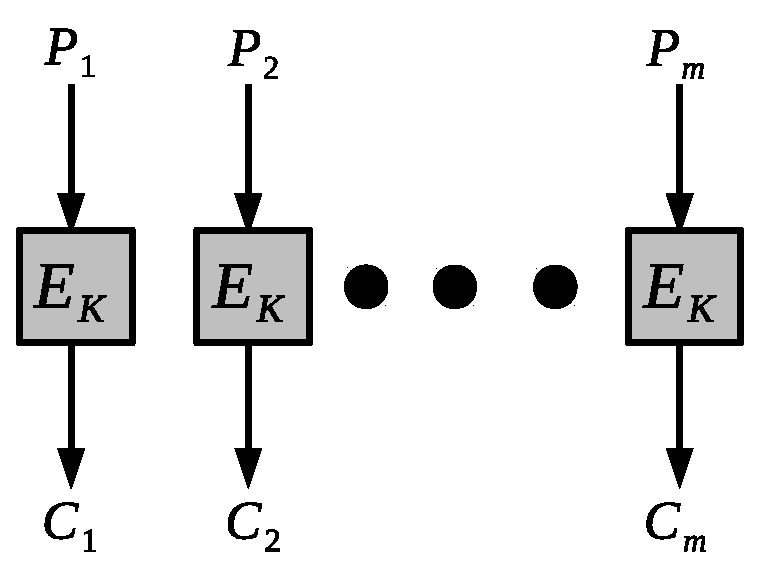
\includegraphics[width=5cm]{images/ecb.eps}}\\

\end{column}
\end{columns}

\pause
\vspace{0.5cm}

$$Pr[\mathbf{Exp}_{\cal SE}^{ind-cpa-1}(A)=1]=1$$ y

$$Pr[\mathbf{Exp}_{\cal SE}^{ind-cpa-0}(A)=1]=0$$


}

\frame
{
	
\frametitle{Seguridad de CBC IV=Contador}
\begin{columns}
\begin{column}{5cm}
	 \begin{small}

	 \begin{tabular}{l}
	 \textbf{Adversario} $A^{{\cal E}_K(LR(\cdot,\cdot,b))}$ \\
	 \tab $M_{0,1}\leftarrow 0^{n}$;$M_{1,1}\leftarrow 0^n$\\
	 \tab $M_{0,2}\leftarrow 0^{n}$;$M_{1,2}\leftarrow 0^{n-1}1$\\
	 \tab $IV_1,C[1] \leftarrow {\cal E}_K(LR(M_{0,1},M_{1,1},b))$\\
	 \tab $IV_2,C[2] \leftarrow {\cal E}_K(LR(M_{0,2},M_{1,2},b))$\\

	 \tab \textbf{if} $C[1]=C[2]$, \textbf{then}\\
	 \tab\tab \textbf{return} 1\\
	 \tab \textbf{else}\\
	 \tab\tab \textbf{return} 0\\ 
	 \end{tabular}\\	 
	 \end{small}
	 \end{column}
\begin{column}{5cm}	

\framebox{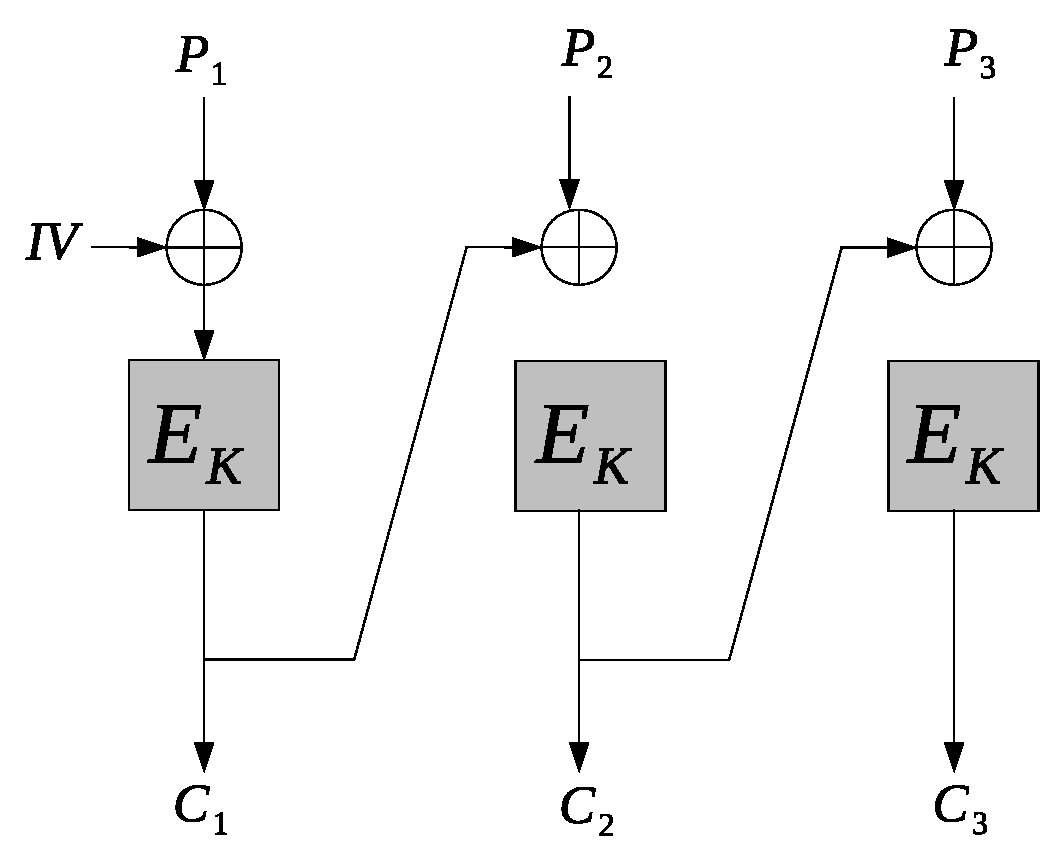
\includegraphics[width=5cm]{images/CBC.eps}}\\

\end{column}
\end{columns}

\vspace{0.5cm}

$$Pr[\mathbf{Exp}_{\cal SE}^{ind-cpa-1}(A)=1]=1$$ y

$$Pr[\mathbf{Exp}_{\cal SE}^{ind-cpa-0}(A)=1]=0$$


}


\frame
{
	
\frametitle{Seguridad de CBC IV=Contador}
\begin{columns}
\begin{column}{5cm}
	 \begin{small}

	 \begin{tabular}{l}
	 \tab si $b=0$:\\
	 \tab \tab $IV_1=0$ y $IV_2=1$,\\
	 \tab \tab $C_1=E_K(0)$ y $C_2=E_K(1)$.\\
	 \tab si $b=1$:\\
	 \tab \tab $IV_1=0$ y $IV_2=1$,\\
	 \tab \tab $C_1=E_K(0)$ y $C_2=E_K(0)$.\\
	 \end{tabular}\\	 
	 \end{small}
	 \end{column}
\begin{column}{5cm}	

\framebox{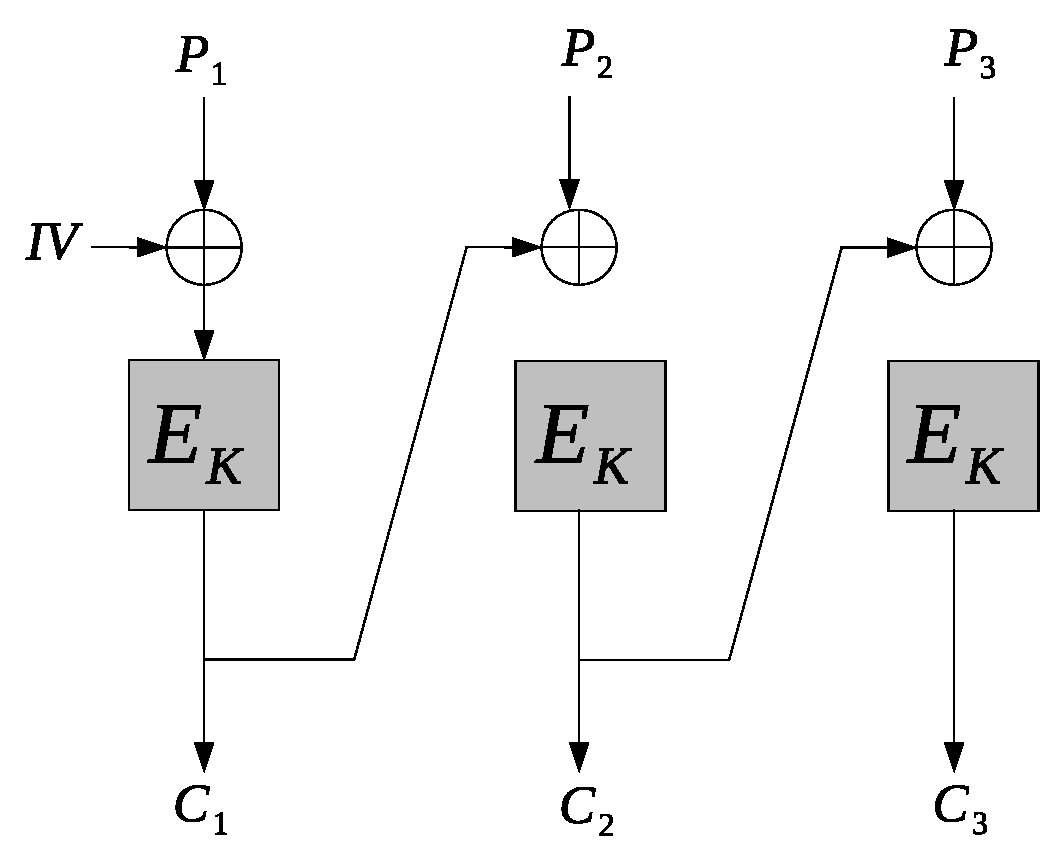
\includegraphics[width=5cm]{images/CBC.eps}}\\

\end{column}
\end{columns}

\vspace{0.5cm}
}

\frame
{
\frametitle{Seguridad de red de Feistel 1 ronda}
\begin{columns}
\begin{column}{6cm}<2>
	 \begin{small}
	 \begin{tabular}{l}
	 \textbf{Adversario} $A^{{\cal E}_K(LR(\cdot,\cdot,b))}$\\
	 \tab $L_{0,1}\leftarrow 0^{n/2}$;$R_{1,1}\leftarrow 1^{n/2}$;$M_0 \leftarrow L_{0,1}||R_{0,1}$\\
	 \tab $L_{0,2}\leftarrow 0^{n/2}$;$R_{1,1}\leftarrow 0^{n/2}$;$M_1 \leftarrow L_{1,1}||R_{1,1}$\\
	 \tab $C_1 \leftarrow {\cal E}_K(LR(M_{0},M_{1},b))$\\
	 \tab $L_1||R_1=C_1$\\
	 \tab \textbf{if} $L_1=0^{n/2}$, \textbf{then}\\
	 \tab\tab \textbf{return} 1\\
	 \tab \textbf{else}\\
	 \tab\tab \textbf{return} 0\\ 
	 \end{tabular}\\	 
	 \end{small}
	 \end{column}
\begin{column}{4cm}<1,2>	

\framebox{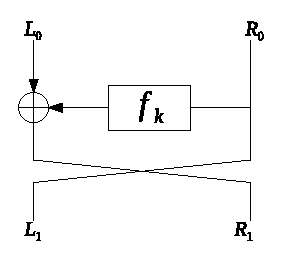
\includegraphics[width=4cm]{images/FN_1r.eps}}\\

\end{column}
\end{columns}
}

\frame
{
\frametitle{Otra definición}

Indistinguibilidad de cadenas aleatorias.


$$Adv_{{\cal E}_K}^{ind\$}({\cal A})=\left| Pr \left[ K \stackrel{\$}{\leftarrow}{\cal K}: {\cal A}^{{\cal E}_K}=1 \right]-Pr \left[ {\cal A}^{\$(\cdot,\cdot)}=1 \right]\right|$$

\vspace{0.5cm}

{\color{red} $\$(\cdot,\cdot)$ es un oráculo que regresa cadenas de bits aleatorios}


}

\frame
{
\frametitle{Seguridad de red de Feistel 1 ronda}
\begin{columns}
\begin{column}{6cm}<2>
	 \begin{small}
	 \begin{tabular}{l}
	 \textbf{Adversario} ${\cal A}^{{\cal E}_K((L_{0},R_{0}))}$\\
	 \tab $L_1 \leftarrow R_0$\\
	 \tab $R_1 \leftarrow L_0 \oplus f_k(R_0)$\\
	 \tab \textbf{if} $L_1=R_0$, \textbf{then}\\
	 \tab\tab \textbf{return} 1\\
	 \tab \textbf{else}\\
	 \tab\tab \textbf{return} 0\\ 
	 \end{tabular}\\	 
	 \end{small}
	 \end{column}
\begin{column}{4cm}<1,2>	

\framebox{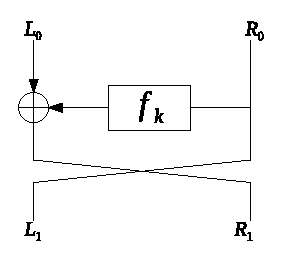
\includegraphics[width=4cm]{images/FN_1r.eps}}\\

\end{column}
\end{columns}
\vspace{1cm}

\pause

$$Adv_{{\cal E}_K}^{ind\$}({\cal A})=1-\frac{1}{2^{(n/2)}}$$


}


\frame
{
\frametitle{Seguridad de red de Feistel 2 rondas}
\begin{columns}
\begin{column}{6cm}
	 \begin{small}
	 \begin{tabular}{l}
 	 \tab \textbf{Entrada:} $(L_0,R_0)$\\	 
	 \tab $L_1 \leftarrow L_0 \oplus f_k(R_0)$\\
	 \tab $R_1 \leftarrow R_0 \oplus f_k(f_k(L_0 \oplus f_K(R_0))$\\
     \hline	 
	 \tab \textbf{Entrada:} $(L_1,R_0)$\\	 
	 \tab $L_2 \leftarrow L_1 \oplus f_k(R_0)$\\
	 \tab $L_2 \leftarrow [L_0 \oplus f_k(R_0)]\oplus f_k(R_0)$\\
	 \tab $L_2 \leftarrow L_0$\\
	 \end{tabular}\\	 
	 \end{small}
	 \end{column}
\begin{column}{4cm}	

\framebox{\includegraphics[width=3cm]{images/FN_2r.eps}}\\

\end{column}
\end{columns}
}

\frame
{
\frametitle{Feistel 3 rondas}
\begin{columns}
\begin{column}{6cm}
	 \begin{small}
	 \begin{tabular}{l}
 	 \tab \textbf{Entrada:} $(L_0,R_0)$\\	 
 	 \tab $L_1 \leftarrow R_0 \oplus f_k(f_k(L_0 \oplus f_K(R_0))$\\
	 \tab $R_1 \leftarrow L_0 \oplus f_k(R_0) \oplus $\\
	 \tab\tab$f_k(R_0 \oplus f_k(f_k(L_0 \oplus f_K(R_0)))$\\
	 \end{tabular}\\	 
	 \end{small}
	 \end{column}
\begin{column}{4cm}	

\framebox{\includegraphics[width=3cm]{images/FN_3r.eps}}\\

\end{column}
\end{columns}
}

\frame
{
\frametitle{Modo contador}
\begin{columns}
\begin{column}{6cm}<2>
	 \begin{small}
	 \begin{tabular}{l}
 	 \tab $IV^1=0$,$P_1^1=0^n$,$P_2^1=1^n$\\
 	 \tab $C_1^1=0^n\oplus E_K(0)$,$C_2^1=1^n\oplus E_K(1)$\\
 	 \\
 	 \tab $IV^2=1$,$P_1^2=1^n$,$P_2^2=0^n$\\
 	 \tab $C_1^2=1^n\oplus E_K(1)$,$C_2^2=0^n\oplus E_K(2)$\\
 	 \\
 	 \tab $C_1^2=C_2^1$.
	 \end{tabular}\\	 
	 \end{small}
	 \end{column}
\begin{column}{4cm}<1,2>	

\framebox{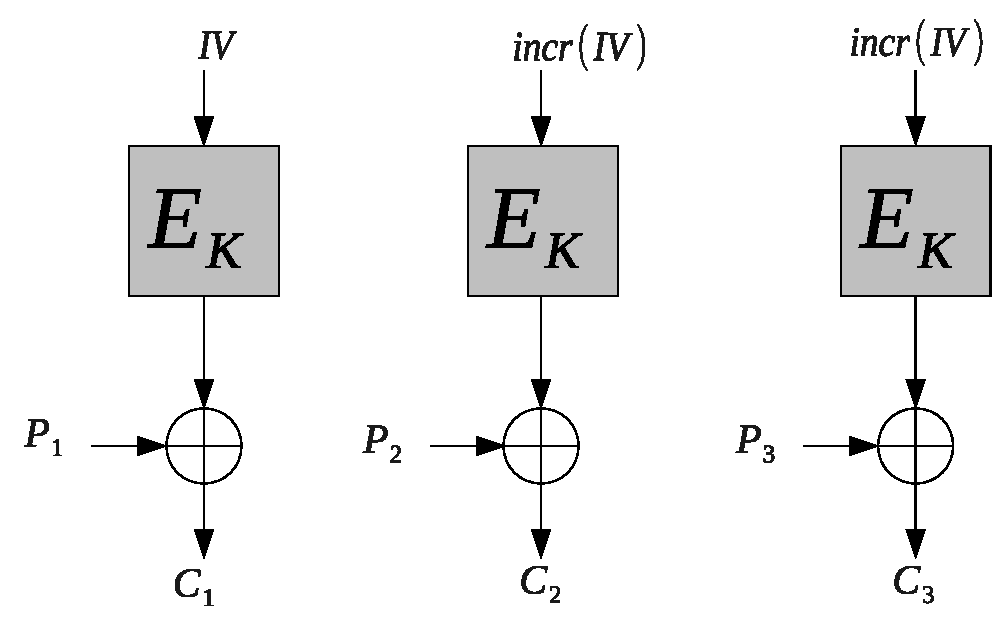
\includegraphics[width=4cm]{images/ctr.eps}}\\
\vspace{0.5 cm}
$inc(IV)=IV++$
\end{column}
\end{columns}
\pause
\vspace{0.5cm}
{\color{red} $IV=(nonce||ctr)$,$|nonce|=96$ bits, $|ctr|=32$.}

}

\frame
{
	\frametitle{Lemma PRP/PRF}
	
	Para la demostración de usa una técnica conocida como interacción con juegos.\\\vspace{0.5cm}
\begin{center}
\begin{small}
\framebox{
\begin{tabular}{l}
\textbf{01} $bad\leftarrow false$; \textbf{for} $X\in\binStr^n$ \textbf{do} $\pi(X)\leftarrow undef$\\
\\
\textbf{When} $A$ \textbf{asks query} X:\\  
\textbf{10} $Y\rand \binStr^n$\\
\textbf{11} \textbf{if} $Y \in Range(\pi)$ \textbf{then}  $bad\leftarrow true$\\
\textbf{12} \tab\fbox{$Y \rand \overline{Range(\pi)}$}\\
\textbf{13} $\pi(X) \leftarrow Y$\\
\textbf{14} \textbf{Return $Y$}\\
\end{tabular}
}\\
\vspace{0.2 cm}
Descripción de Juego $P$, para el juego $R$ sólo de remueve lo que hay dentro del rectángulo. 

\end{small}

\end{center}
}

\frame
{
	\frametitle{Lemma PRP/PRF}
	
	\begin{itemize}
	\item El juego $P$ reproduce una permutación aleatoria.\\
	\item El juego $R$ reproduce una función aleatoria.\\
\end{itemize}		
	
	$$Pr\left[ A^{\rho}\Rightarrow 1\right] -
	         Pr\left[ A^{\pi} \Rightarrow 1\right] $$
	         
	$$Pr\left[ A^{\rho}\Rightarrow 1\right] = Pr[A^{Game\,R}] $$
	$$Pr\left[ A^{\pi }\Rightarrow 1\right] = Pr[A^{Game\,P}] $$
	
	Entonces
	
	$$ Pr\left[A^{Game R}\right] - Pr\left[A^{Game\,P}\right] \leq Pr\left[A^{Game\,R}\,sets\,bad\right]$$ 
}

\frame 
{
	\frametitle{Lemma PRP/PRF}

Si pensamos en que las consultas del adversario son cadenas de $n$ bits.\\

La única manera para distinguir entre ambos juegos es que el valor seleccionado en $Y\leftarrow \binStr^n$ se encuentre en $Range(\pi)$, en ese caso la bandera $bad\leftarrow true$.

Cada vez que se hace una consulta el conjunto $Rand(\pi)$ se va formando, es decir:\\
\vspace{0.5cm}
\begin{tabular}{lll}
$Pr[Y \in Range(\pi)]=0/2^n$ & $|Range(\pi)|=0$ & 1\\
$Pr[Y \in Range(\pi)]=1/2^n$ & $|Range(\pi)|=1$ & 2\\
$Pr[Y \in Range(\pi)]=2/2^n$ & $|Range(\pi)|=2$ & 3\\
$Pr[Y \in Range(\pi)]=3/2^n$ & $|Range(\pi)|=3$ & 4\\
... & & \\
$Pr[Y \in Range(\pi)]=(q-1)/2^n$ & $|Range(\pi)|=q-1$ & q\\

\end{tabular}


}

\frame 
{
	\frametitle{Lemma PRP/PRF}
	
	Entonces haciendo $q$ consultas:\\
	
	\begin{align*}
	Pr\left[A^{Game\,R}\,sets\,bad\right]\leq&\frac{0}{2^n}+\frac{1}{2^n}+\frac{2}{2^n}+...+\frac{q-1}{2^n}\\
	\leq & \frac{0+1+2+3+...+(q+1)}{2^n}\\
	\leq & \frac{q(q-1)}{2}\frac{1}{2^n}\\
	\leq & \frac{q(q-1)}{2^{n+1}}
	\end{align*}
	
	$$Pr\left[ A^{\rho}\Rightarrow 1\right] -
	         Pr\left[ A^{\pi} \Rightarrow 1\right] \leq \frac{q(q-1)}{2^{n+1}} $$
}

\frame
{
	\frametitle{Lemma PRP/PRF}
	
	Otra forma:\\
	
	Si
	
	\begin{equation*}
	Pr\left[ \pi(X_1)=Y\,and\,\pi(X_2)=Y \right] = \left\{ \begin{array}{ccc}
	0 & si & X_1\neq X_2\\
	2^{-n} & si & X_1 = X_2\\
	\end{array}
\right.
    \end{equation*}	 
\pause

Buscamos colisiones, es decir, parejas iguales de $Y_i,Y_j$, $i\neq j$ en un conjunto de $q$ valores.\\

\pause

$$  \displaystyle{\binom{q}{2} = \frac{q!}{2!(q-2)!}}$$\\

Para cada pareja la probabilidad de ocurrencia es de $2^{-n}=1/2^n$.

}

\frame
{
	\frametitle{Lemma PRP/PRF}
\begin{align*}
 \displaystyle{\binom{q}{2} \cdot \frac{1}{2^n}} =& \frac{q!}{2!(q-2)!}\cdot\frac{1}{2^n}\\ \\\pause
=& \frac{q(q-1)(q-2)!}{2(q-2)!}\cdot\frac{1}{2^n}\\ \\
=& \frac{q(q-1)}{2} \cdot\frac{1}{2^n}\\ \\
=& \frac{q(q-1)}{2} \cdot\frac{1}{2^n}\\ \\
=& \frac{q(q-1)}{2^{n+1}}\\ \\
\end{align*}
}

\frame
{
	\frametitle{Ataque del cumpleaños}

Tenemos la función $E:\binStr^k \times \binStr^n \rightarrow \binStr^n$ y un oráculo $g:\binStr^n \rightarrow \binStr^n$ que es una instancia de $E$ o una función aleatoria.\\
\begin{itemize}
\item Consultando al oráculo $g$ con valores diferentes $x_1,x_2,...,x_q$ se obtiene $y_1,y_2,...,y_q$.\\


\item Si $g$ es una permutación todos los valores $y_1,y_2,...,y_q$ serán diferentes.


\item Si $g$ es una función todos los valores $y_1,y_2,...,y_q$ pueden o no ser diferentes.


\item Un adversario eficiente puede tomar $q=\sqrt{2^n}=2^{n/2}$ consultas para distinguir entre un cifrador por bloques y una función aleatoria.
\end{itemize}\pause

{\color{red} Este resultado se debe a la paradoja del cumpleaños.}

}

\frame
{
	\frametitle{Seguridad de cifradores por bloque}


$$\mathbf{Adv}_{E}^{prf}\geq 0.3\cdot \frac{q(q-1)}{2^n} $$

\textbf{Demostración:}\\

Recordemos que la probabilidad de encontrar al menos una colisión en $N$ elementos es:\\
$$C(N,q)=\frac{q(q-1)}{2N}$$

Se va a encontrar la cota inferior, es decir, la probabilidad de que no haya colisiones hasta las $q$ consultas.\\

La probabilidad de que no se hayan encontrado colisiones hasta la consulta $i+1$ es:\\

$$Pr\left[ D_{i+1}|D_i\right]=\frac{N-i}{N}=1-\frac{i}{N}$$\\

hay que notar que $Pr[D_1] = 1$, es decir la primera consulta. 
}

\frame
{
	\frametitle{Seguridad de cifradores por bloque}

	La probabilidad de no encontrar colisiones se puede calcular como:\\
	
	\begin{align*}
    1-C(n,q) = & Pr\left[D_q\right]\\
             = & Pr\left[D_q|D_{q-1}\right]\cdot Pr\left[D_q\right]\\
             = & \prod_{i=1}^{q-1} Pr\left[D_{i+1}|D_{i}\right]\\
             = & \prod_{i=1}^{q-1} \left(1-\frac{i}{N}\right).\\
	\end{align*}

Usando la desigualdad siguiente:\\

$$\left(1 - \frac{1}{e} \right) \cdot x \leq 1 - e^{-x} \leq x.$$

}

\frame
{

	\frametitle{Seguridad de cifradores por bloque}
	\begin{align*}
              = & \prod_{i=1}^{q-1} \left(1-\frac{i}{N}\right).\\
	\end{align*}

Usando la desigualdad $1-x \leq e^{-x}$, tenemos:\\

$$\prod_{i=1}^{q-1} e^{-1/N}=e^{-\frac{1}{N}-\frac{2}{N}-...-\frac{(q-1)}{N}}=e^{-\frac{q(q-1)}{2N}},$$

Ahora:\\

$$C(N,q)\geq  1 -   e^{-\frac{q(q-1)}{2N}}$$

}

\frame
{

	\frametitle{Seguridad de cifradores por bloque}
$$C(N,q)\geq  1 -   e^{-\frac{q(q-1)}{2N}}$$

Sabemos que $q(q-1)/2N\leq 1$ porque $q \leq \sqrt{2N}$, asando la desigualdad:
$$1-e^{-x}\geq (1-e^{-1})\cdot x$$
\begin{align*}
C(N,q)\geq &\left( 1 - \frac{1}{e} \right) \cdot  \frac{q(q-1)}{2^n}\\
      \geq &  0.63 \cdot  \frac{q(q-1)}{2N}\\ 
      C(N,q)\geq & 0.3 \cdot  \frac{q(q-1)}{N}
\end{align*}

}

\frame
{
	\frametitle{Códigos de autenticación de mensajes (MAC)}
	
\begin{itemize}
\item En algunas aplicaciones la información es pública, es decir, no requiere privacidad.\\
\item Un aspecto importante es garantizar que la información que se recibe es efectivamente la que fue enviada y también verificar su origen.\\
\item Autenticación e integridad de datos.
\end{itemize}	
}

\frame
{
	\frametitle{Códigos de autenticación de mensajes (MAC)}
	
\begin{itemize}
\item Inicialmente debe existir una llave secreta compartida $K$.\\
\item El emisor del mensaje $M$ calcula una etiqueta como $\tau=MAC_K(M)$, envía la pareja $(M,\tau)$.\\
\item Los receptores reciben $(M,\tau)$, al conocer $K$ pueden calcular $\tau'=MAC_K(M)$, el mensaje es valido sí sólo sí, $\tau=\tau'$. 
\end{itemize}	

{\color{red} ¿En qué casos $\tau\neq \tau'$?}
\pause
\begin{itemize}
\item La llave secreta no es la misma, falla de autenticación.\\ \pause
\item El mensaje recibido fue modificado, falla de integridad de datos. 
\end{itemize}

}

\frame
{
	\frametitle{Códigos de autenticación de mensajes (MAC)}

Son funciones del tipo 
$$\binStr^* \times \binStr^K \rightarrow \binStr^{\ell}$$

\begin{itemize}
\item $\ell$ es el tamaño de la etiqueta y generalmente es un valor pequeño 64,96,128 bits.
\item $K$ es el tamaño de la llave.
\end{itemize}

}

\frame
{
	\frametitle{¿Cómo construir una MAC?}

\begin{itemize}
\item Modos de operación de cifradores por bloque.
\item Permutaciones públicas.
\item Funciones hash universales y una fuente de pseudoaleatoriedad.
\end{itemize}

}


\frame
{
	\frametitle{CBC}
\begin{center}
\framebox{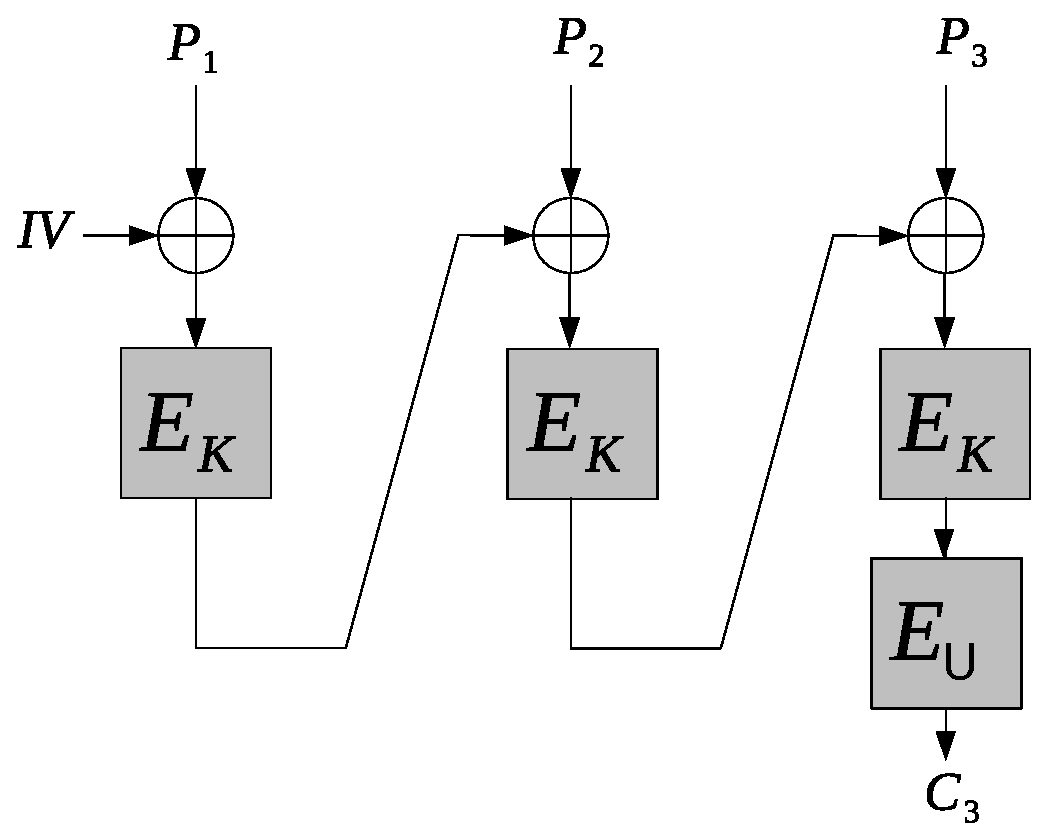
\includegraphics[width=6cm]{images/CBCMAC.eps}}\\
\end{center}

$CBC$ con una llamada extra a un cifrador con una llave diferente.

}

\frame
{
	\frametitle{Funciones hash universales y xor universales}

Para $x_1,x_2 \in \binStr^{nm}$ y $x_1 \neq x_2$:

$$Pr[h\leftarrow \binStr^n ;F_h(x_1)=F_h(x_2)]=\epsilon$$

$$Pr[h\leftarrow \binStr^n,a\leftarrow \binStr^n ;F_h(x_1)\oplus F_h(x_2)=a]=\epsilon$$

\vspace{1cm}
Si $\epsilon = 1/2^n$ la función es universal, y si $\epsilon>0$ pero es un valor despreciable, la función es casi universal (almost universal).

}

\frame
{
	\frametitle{Constricción de Wegman y Carter}
	
	$$MAC_{K,h}(M,nonce)=H_h(M) \oplus E_K(nonce)$$
	
	\begin{itemize}
	\item Dos llaves $K$ y $h$.
	\item $H_h(\cdot)$ es una función hash xor universal.
	\item $E_K(\cdot)$ puede ser una cifrador por bloques.
	\item El $nonce$ debe ser único para cada mensaje.
	\end{itemize}


}

\frame
{

\frametitle{Seguridad de una MAC}

Sea $\phi$ una MAC,  se dice que es segura si la siguiente probabilidad es muy pequeña:

$${\bf Adv}_{\Psi}^{auth}(A)= \Pr [A^{{\cal E}_K(.,.,.)} \mbox{ forges }]$$
	
	{\color{blue}Es muy difícil para el adversario construir un par de mensaje y etiqueta que verifique sin conocer la llave secreta.}\\
}

\frame
{

	\frametitle{MAC insegura}	
	
	\begin{center}
	\framebox{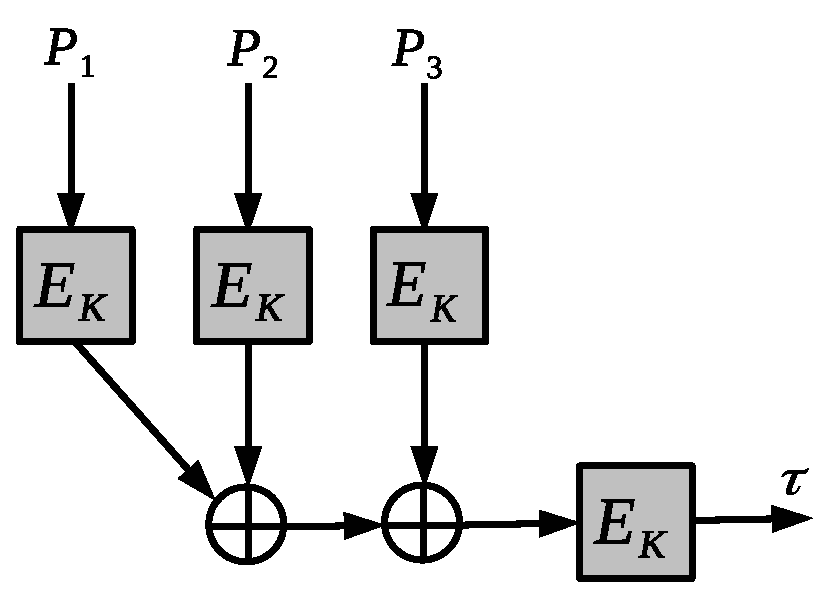
\includegraphics[width=4cm]{images/mac_in.eps}}\\
	\end{center}
	
	$$MAC_K(P_1,P_2,P_3)=E_K(E_K(P_1)\oplus E_K(P_2) \oplus E_K(P_3))$$

{\color{red}¿porqué insegura?}

\pause

$$MAC_K(P_1,P_2,P_3)=MAC_K(P_1,P_3,P_2)=MAC_K(P_3,P_2,P_1)$$

}

\frame
{
\frametitle{Hash polinomial} 
	
Una función:

$$ H:\{0,1\}^n \times \{0,1\}^{nm} \rightarrow \{0,1\}^n $$

definida como:

$$H_h(P_1||...||P_m) = P_1h^m \oplus P_2h^{m-1} \oplus ... \oplus P_mh$$

Todas las operaciones son en $GF(2^n)$,$h,P_i \in \{0,1\}^n$.\\

Es una función $AXU$ (almost xor universal hash),ya que $G \in \{0,1\}^n$, y $P\neq P'$.\\
$$\Pr[h\rand\{0,1\}^n:H_h(P) \oplus H_h(P^{'})=G] \leq \frac{ maxdegree(P,P^{'})}{2^n}$$

}


\frame{
\frametitle{Multilinear Universal Hash}

A MLUH (Multilinear Universal Hash) with data path $d$ takes in a message $M=M_1||M_2||\cdots||M_m \in \{0,1\}^{dm}$, where each
 $|M_i|=d$. MLUH  produces a $td$ bit output for some $t\geq 1$. To do this MLUH requires $(m+t-1)d$ bits of key material.
 Assuming that $K = K_1||K_2||\ldots||K_{m+t-1}$, where each $|K_i|=d$ we define
 $${\sf MLUH}^{d,t}_K(M) = h_1||h_2||\cdots||h_t,$$
 where
 \begin{eqnarray}
h_1 & = & M_1\cdot K_1 \oplus M_2\cdot K_2 \oplus ...\oplus M_m\cdot K_m \nonumber \\
h_2 & = & M_1\cdot K_2 \oplus M_2\cdot K_3 \oplus ...\oplus M_m\cdot K_{m+1}\nonumber\\
.   & & \nonumber \\
.   & & \nonumber \\
.   & & \nonumber \\ \label{eq:mluh}
h_t & = & M_1\cdot K_t \oplus M_2\cdot K_{t+1} \oplus ....\oplus M_m\cdot K_{t+m-1},\nonumber
\end{eqnarray}
and the additions and multiplications are in the field GF($2^d$).

}

\frame{
\frametitle{Multilinear Universal Hash}
As the name suggest, the {\sf MLUH} is a universal hash function, more specifically it has low differential probabilities.
For a randomly chosen key $K$ from the key space $\{0,1\}^{d(t+m-1)}$, and any pair of distinct messages $M_1,M_2 \in \{0,1\}^{md}$ and a $\delta \in \{0,1\}^{dt}$,
\begin{equation}
\Pr[{\sf MLUH}^{d,t}_K(M_1) \oplus {\sf MLUH}^{d,t}_K(M_2) = \delta] \leq \frac{1}{2^{dt}}
\end{equation}
where the probability is taken over the uniform random choice of the key $K$.
}

\frame
{
\frametitle{Una PRF como un MAC}

Sea $F:{\cal K} \times {\cal D} \rightarrow \binStr^{\tau}$ una familia de funciones, asociamos a $F$ un código de autenticación de mensajes $MAC:{\cal K} \times {\cal D} \rightarrow \binStr^{\tau}$ de la siguiente manera:\\
\vspace{1 cm}
\begin{tabular}{l}
\textbf{Algorithm}$MAC_K(M)$\\
\tab \textbf{if} $M \neq {\cal D}$ \textbf{then return} $\bot$\\
\tab$T\leftarrow F_K(M)$\\
\tab\textbf{return} T
\end{tabular}

}

\frame
{
	\frametitle{Cifrado autenticado}
	
	Después de haber visto algoritmos de cifrado y MACs, podemos hacer una composición genérica de ambas:\\	
	
	\begin{itemize}
	\item Cifrar y MAC, $\overline{{\cal E}}={\cal E}(K_e,M)||MAC(Ka,M))$. \\
	\item MAC después cifrar, $\overline{{\cal E}}={\cal E}(K_e,M||MAC(Ka,M))$\\
	\item Encrypt después MAC, $\overline{{\cal E}}={\cal E}(K_e||K_a,M)=C||MAC(Ka,C))$ donde $C={\cal E}(K_m,M)$\\
	\end{itemize}

}

\frame
{
	\frametitle{Ataques de mensaje cifrado seleccionado}
	
	\begin{itemize}
	\item El adversario es un algoritmo probabilístico.
	\item El adversario interactúa con oráculos.
	\item En este caso el adversario tiene acceso a $E_K(\cdot)$ y a $E^{-1}_K(\cdot)$.
	\item No se puede consultar $E^{-1}_K(\cdot)$ con un resultado obtenido previamente con $E_K(\cdot)$, y viceversa.
	\item El ataque es adaptativo, es decir, el adversario puede construir su próxima consulta en base a los resultados de las consultas previas.
	\end{itemize}
	
}

\frame
{
	\frametitle{Ataque al modo contador}

\begin{columns}
\begin{column}{5cm}
	 \begin{small}

	 \begin{tabular}{l}
	 \textbf{Adversario} $A^{{\cal E}_K(LR(\cdot,\cdot),{\cal E}^{-1}_K(\cdot)}$ \\
	 \tab $M_{0}\leftarrow 0^{n}$;$M_{1}\leftarrow 1^n$\\
	 \tab $r,C \leftarrow {\cal E}_K(LR(M_0,M1,b)$\\
	 \tab $C'\leftarrow C \oplus 1$\\
	 \tab $M\leftarrow {\cal E}^{-1}_K(C')$\\
	 \tab \textbf{if} $M=M_0$, \textbf{then}\\
	 \tab\tab \textbf{return} 1\\
	 \tab \textbf{else}\\
	 \tab\tab \textbf{return} 0\\ 
	 \end{tabular}\\	 
	 \end{small}
	 \end{column}
\begin{column}{5cm}	

\framebox{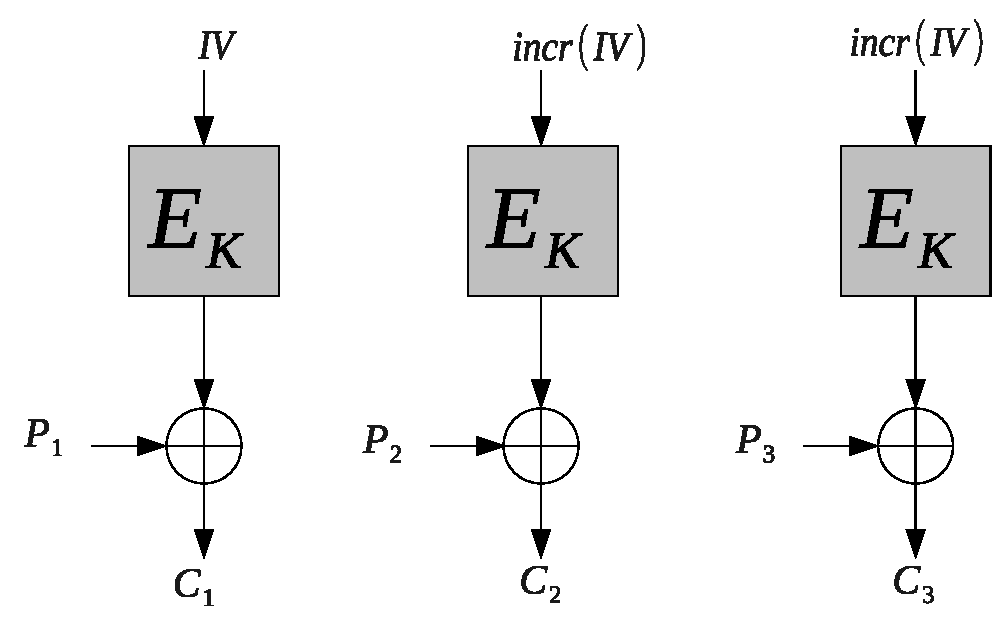
\includegraphics[width=5cm]{images/ctr.eps}}\\

\end{column}
\end{columns}

\vspace{0.5cm}

$$Pr[\mathbf{Exp}_{\cal SE}^{ind-cca-1}(A)=1]=1$$ y

$$Pr[\mathbf{Exp}_{\cal SE}^{ind-cca-0}(A)=1]=0$$


}

\frame
{
	\frametitle{Ataque al modo contador}

\begin{columns}
\begin{column}{5cm}
	 \begin{small}

	 \begin{tabular}{l}
	 \tab $M_{0}\leftarrow 0^{n}$;$M_{1}\leftarrow 1^n$\\
	 \tab \textbf{if} $b=0$ \textbf{then}\\
	 \tab\tab $C\leftarrow {\cal E}(r)$\\
	 \tab \textbf{else}\\
	 \tab \tab $C\leftarrow {\cal E}(r) \oplus 1^n$\\
	 \hline
	 \tab $C'\leftarrow C \oplus 1^n$\\
	 \tab $M\leftarrow {\cal E}^{-1}_K(C')$\\
	 \tab \textbf{if} $M_0$ \textbf{then}\\
	 \tab\tab $M\leftarrow {\cal E}_K(r) \oplus {\cal E}(r) \oplus 1^n$\\
	 \tab \textbf{else}\\
	 \tab\tab $M\leftarrow {\cal E}_K(r)\oplus 1^n \oplus {\cal E}(r) \oplus 1^n$\\
	 \end{tabular}\\	 
	 \end{small}
	 \end{column}
\begin{column}{5cm}	

\framebox{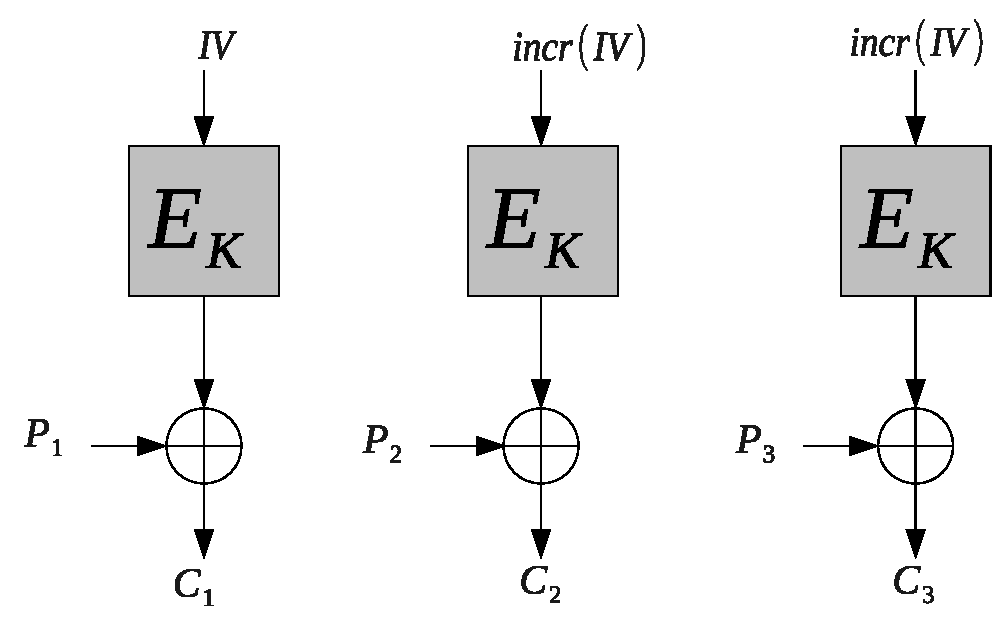
\includegraphics[width=5cm]{images/ctr.eps}}\\

\end{column}
\end{columns}




}




\end{document} 